% REMEMBER: You must not plagiarise anything in your report. Be extremely careful.
\documentclass{l4proj}

    
%==============================================================================
% Put any additional packages here
% You can add any packages you want, as long as it does not alter
% the overall format (e.g. don't change the margins or the reference style).
%
\usepackage{pdfpages} % if you want to include a PDF for an ethics checklist, for example
\usepackage{multirow}
%
%

\begin{document}

%==============================================================================
%% METADATA
\title{Virtual Reality Visual Field Testing Device} % change this to your title
\author{Mok Kah Hou}
\date{October 30, 2024}

\maketitle

%==============================================================================
%% ABSTRACT
\begin{abstract}
    This project presents the design, implementation, and evaluation of a virtual reality (VR)-based visual field testing system using consumer-grade VR hardware with integrated eye tracking. Traditional perimetry devices like the Humphrey Visual Field Analyser are limited by their size, cost, and clinical requirements. In contrast, this system aims to provide a more accessible and portable alternative suitable for use in remote or non-clinical environments.

    The application was developed using Unity, following a Model-View-Controller structure. It features static stimulus detection, real-time fixation feedback, and structured post-test data logging. Users undergo short test sessions during which peripheral stimuli are flashed, and responses are recorded using the space-bar key. A Python-based post-test script automatically analyses the raw data and compiles a clinical-style PDF report, including a greyscale visual field map, gaze density map, false positive scatter plot, and key performance metrics.
    
    Evaluation was conducted through a user study with 12 participants. Quantitative analysis revealed that the inclusion of real-time visual fixation feedback significantly improved centre fixation consistency ($p \approx 0.017$) and reduced false positives ($p \approx 0.015$), though it also increased reaction time ($p \approx 0.018$). Subjective feedback using SSQ and NASA-TLX questionnaires indicated that the system was generally well-tolerated, with only moderate symptoms such as eye strain and fatigue reported.
    
    The results suggest that VR-based perimetry is a viable approach for preliminary visual field screening and has the potential for broader application in remote or mobile healthcare settings. The system also provides an extensible framework for future development, such as adaptive stimulus strategies or even integration into clinical workflows.

\end{abstract}


%==============================================================================
%% ACKNOWLEDGEMENTS
\chapter*{Acknowledgements}

% Enter any acknowledgements here. This is optional; you may leave this blank if you wish.
% or remove the entire chapter
%
% We give thanks to the Gods of LaTeX, who in their eternal graciousness, 
% have granted that this document may compile without errors or overfull hboxes.
%

I would like to sincerely thank my project partner, Nik Harith, for his support, collaboration, and valuable input throughout this project. Working together made the process more enjoyable and helped push the system further than I could have managed alone.

I am also grateful to my supervisor, Dr. Paul Siebert, for his guidance and feedback at every stage. His insights were instrumental in shaping both the technical and research direction of this work.

%==============================================================================

% EDUCATION REUSE CONSENT FORM
% If you consent to your project being shown to future students for educational purposes
% then insert your name and the date below to sign the educational use form that appears in the front of the document. 
% You must explicitly give consent if you wish to do so.
% If you sign, your project may be included in the Hall of Fame if it scores particularly highly.
%
% Please note that you are under no obligation to sign 
% this declaration, but doing so would help future students.
%
\def\consentname {Mok Kah Hou} % your full name
\def\consentdate {30 October 2024} % the date you agree
%
\educationalconsent


%==============================================================================
\tableofcontents

%==============================================================================
%% Notes on formatting
%==============================================================================
% The first page, abstract and table of contents are numbered using Roman numerals and are not
% included in the page count. 
%
% From now on pages are numbered
% using Arabic numerals. Therefore, immediately after the first call to \chapter we need the call
% \pagenumbering{arabic} and this should be called once only in the document. 
%
%
% The first Chapter should then be on page 1. 

% PAGE LIMITS
% You are allowed 40 pages for a 40 credit project and 30 pages for a 
% 20 credit report. 
% This includes everything numbered in Arabic numerals (excluding front matter) up
% to but *excluding the appendices and bibliography*.
%
% FORMATTING
% You must not alter text size (it is currently 10pt) or alter margins or spacing.
% Do not alter the bibliography style. 
%
%==================================================================================================================================
%
% IMPORTANT
% The chapter headings and structure here are **suggestions**. You don't have to follow this model if
% it doesn't fit your project. Every project should have an introduction and conclusion,
% however.  If in doubt, your supervisor can give you specific guidance; their view takes precedence over
% the structure suggested here.
%
%==================================================================================================================================
\chapter{Introduction}

% reset page numbering. Don't remove this!
\pagenumbering{arabic} 

\section{Motivation}
 

This dissertation presents a VR-based visual field testing (VFT) system, designed to produce visual field-testing results that, in future iterations, may approach the standard of traditional perimetry while offering greater accessibility and flexibility. 

Visual field loss is a symptom in a wide range of ocular and neurological disorders, such as glaucoma and hemianopia. These conditions can result in scotomas (blind spots), tunnel vision, or even permanent blindness, with up to 53\% of glaucoma cases going undiagnosed in underdeveloped countries \citep{mot1}. Early-stage defects are often hard to notice, but if detected and treated promptly, the progression of vision loss can often be slowed, stopped, or even compensated using visual rehabilitation techniques \citep{mot2}. The consequences of missed diagnoses are severe, such as loss of independence, employment, and overall quality of life. Therefore, the ability to detect visual defects early can have life-changing implications for the patient. 

However, traditional perimetry systems, such as the Humphrey Visual Field Analyser (HFA) and the Optos Daytona, are significant investments for medical practices. For instance, the Zeiss Humphrey Field Analyser 3 (HFA3) is listed at \$8,393 \footnote{\href{www.ophthalmetryoptical.com/retinal-cameras/zeiss-hfa3.html}{www.ophthalmetryoptical.com/retinal-cameras/zeiss-hfa3.html}}, while the Optos Daytona is priced up to \$85,000 \footnote{\href{https://reviewob.com/the-3-most-impactful-technology-additions-to-my-practice/}{www.reviewob.com/the-3-most-impactful-technology-additions-to-my-practice/}}. In contrast, consumer-grade virtual reality (VR) headsets equipped with built-in eye-tracking capabilities are available at substantially lower prices, less than \$600 \footnote{\href{https://www.vive.com/uk/product/vive-pro2/overview/}{www.vive.com/uk/product/vive-pro2/overview/}}. This cost disparity highlights the potential of VR technology to make visual field testing more accessible and affordable.

Furthermore, VR enables immersive environments where fixation can be reinforced in real time, improving test reliability. Visual feedback, head-locked stimuli, and gaze-based feedback can be seamlessly implemented, which are features rarely available in conventional perimetry hardware. Additionally, the software-based nature of VR testing systems makes them inherently more extensible. Researchers can rapidly prototype and evaluate new algorithms and adaptive thresholding models such as ZEST or staircase procedures \citep{mot3} \citep{mot4}. 

Another motivation for this work is to build a transparent and extensible platform that could be shared, forked, and improved by others. Unlike proprietary commercial devices, this system is designed to be modular and openly accessible, promoting collaboration for research, clinical, and educational purposes. Reducing technical and financial difficulties can inspire more vision science innovation, especially in academic institutions or low-resource settings. 

In summary, the motivation behind this dissertation is both practical and inspirational, I aim to reduce the difficulties to early vision screening, explore the potential of VR in functional diagnostics, and inspire the creation of open-source, adaptable software systems that can be shaped by future researchers. 


\newpage
\section{Aims}


This project aims to design, build, and evaluate a functional VR-based visual field-testing platform that offers a practical, affordable, and extensible alternative to traditional perimetry systems. By using consumer-grade virtual reality hardware with integrated eye tracking and real-time visual feedback, the system presents a solution to the challenges of cost, accessibility, and clinical dependency in vision diagnostics. 

This project has been successful in delivering a fully functional prototype, capable of: 

\begin{itemize}
    \item Presenting randomly distributed visual stimuli within an immersive environment
    \item Recording user responses with millisecond precision
    \item Monitoring and reacting to real-time gaze data from integrated eye tracking,
    \item Logging structured data for post-test visualisation and analysis
    \item Producing clinically inspired visual field maps and performance measures in a standalone PDF report.
\end{itemize}

This work aims to explore how early detection of visual defects can be supported through accessible VR-based testing. While not yet a full clinical replacement, the system shows potential as a preliminary screening tool, particularly for remote or underdeveloped regions. 


\section{Content Outline}

This section provides an outline of this dissertation’s structure, summarising the contents of each chapter: \newline

\begin{itemize}
   

    \item \textbf{Background}: Reviews existing literature on visual defects, conventional and automated visual field testing methods, VR technology in healthcare, simulator sickness, and prior related works. \newline
    
    \item \textbf{Analysis and Requirements}: Defines the problem specifications, the functional and non-functional requirements, the project’s limitations, and any major changes to the initial specifications. \newline

    \item \textbf{Design}: Discusses the overall architecture of the VR application, including core workflow, user interface, the repeated fixed-intensity stimulus algorithm, and generation of a final output (JSON data logs \& PDF). \newline

    \item \textbf{Implementation}: Presents the technical details of the prototype, including hardware specifications, software structure in Unity, relevant scripts (C\#), eye tracking integration, data logging, and PDF generation modules. \newline

    \item \textbf{Evaluation}: Summarises informal observations, pilot tests, user studies, relevant questionnaires (SSQ, NASA-TLX), data analyses, and discussion of results. \newline

    \item \textbf{Conclusion}: Concludes the dissertation with a summary of the project’s accomplishments and findings, and proposes possible future works and improvements for subsequent research or product development. \newline

\end{itemize}


% \item If you are referring to a reference as a noun, then cite it as: ``\citet{Orw68} discusses the role of language in political thought.''
% \item If you are referring implicitly to references, use: ``There are many good books on writing \citep{Orw68, Wil09, Pin15}.''
 
% \footnote{Specifying an online resource like \url{https://developer.android.com/studio}
% in a footnote sometimes makes more sense than including it as a formal reference.}


%==================================================================================================================================
\chapter{Background}

A clear understanding of visual field defects, traditional visual field testing methods, and the capabilities of technologies like virtual reality is needed to motivate and guide this project. This chapter provides the necessary context by outlining relevant medical, technological, research foundations, and prior research, that paved the way for the design of a VR-based visual field testing system.


\section{Visual Defects}

A visual field defect refers to any partial loss or abnormality in a person’s field of vision. These defects can range from small blind spots, to large areas of peripheral or central vision loss, depending on the location and extent of damage of the visual pathway. Visual field defects are symptoms of underlying ocular or neurological disorders, such as glaucoma, stroke, or brain injury. This project focuses on two major categories of visual defects:
\begin{itemize}
    \item Peripheral vision loss, commonly seen in progressive diseases like glaucoma.
    \item Hemifield loss, as seen in post-stroke hemianopia.
\end{itemize}

\subsection{Glaucoma}
Glaucoma is a common eye disorder that involves damage to the optic nerve, typically due to elevated intraocular pressure. Over time, glaucoma can result in peripheral vision loss before affecting central vision, causing irreversible blindness if left undiagnosed and untreated \citep{glaucoma1}. Early detection is crucial, as if it is caught early, treatments can slow or halt the progression of the disease. Visual field tests, such as Humphrey Visual Field (HVF) tests, are used to evaluate the extent of functional impairment caused by the loss of optic nerve fibres, and to guide appropriate treatment. It is also recommended that the visual field tests should be performed at least three times within the first year of the diagnosis \citep{glaucoma2}\citep{glaucoma2a}. It is a common misconception that glaucoma-induced vision loss would be obvious, due to the typical depiction of the visual symptom: seeing through a black tunnel. A study by \citep{glaucoma3} showed that 74\% of affected patients described their visual symptoms as varying degrees of blurriness or missing parts around their peripheral vision, and 26\% of patients were unaware of their vision loss. This further reinforces the importance of regular visual field testing and the importance of it being accessible. Figure of typical visual field loss progression of glaucoma shown at \ref{fig: glaucoma progression}.

\subsection{Hemianopia}
Hemianopia is a visual field defect that results in the loss of vision in half of the visual field in one or both eyes. It is typically caused by damage to the visual pathways, such as the occipital lobe, optic radiations, optic tract, and the optic chiasm \citep{hemanopia1}. This condition is most commonly associated with neurological events such as stroke, traumatic brain injury, or tumours affecting the visual processing regions in the brain \citep{hemanopia1}. Unlike eye diseases that develop gradually, hemianopia can occur suddenly, affecting spatial awareness and the ability to navigate environments safely. Individuals with hemianopia may struggle with tasks such as reading, driving, or just day-to-day life, often without full awareness of their visual deficit. In some cases, patients may even adapt to their field loss unconsciously, by filling in the affected area with visual noise or visual hallucinations, leading to delays in seeking medical attention \citep{hemanopia3}.

Because hemianopia involves a distinct, and often dense visual field loss, visual field tests play a critical role in detecting and characterising the extent of visual impairment. Early and regular visual field tests are essential, not only for initial diagnosis but also for monitoring changes over time and helping rehabilitative strategies, such as hemianopic reading training, and prism glasses \citep{hemanopia4}. Given the subtlety of the symptoms and the differences in patient awareness, consistent access to visual field testing is important for quick intervention. Figure of visual field map of left homonymous hemianopia shown at \ref{fig: hemanopia example}.

\section{Visual Field Testing}

\subsection{History of Visual Field Testing}

The practice of assessing the visual field has evolved over more than a century, advancing in both clinical neurology and ophthalmology. In its earliest stages, visual field testing was conducted through confrontation methods, where the examiner compared the patient’s peripheral vision to their own \citep{vft1}. While simple and still used for basic screening, these methods offered limited sensitivity. The development of quantitative perimetry began in the 19th century with the introduction of hemispherical bowl perimeters, which allowed examiners to measure the extent of visual awareness at various distances from fixation \citep{vft1}.

\subsection{Static and Kinetic Perimetry}
Static perimetry, using fixed light stimuli at various locations, was introduced together with kinetic perimetry, which used moving targets to map out isopters, or areas of equal visual sensitivity.

Kinetic perimetry, such as Goldmann perimetry, involves moving a visual stimulus of fixed intensity and size from non-seeing to seeing areas of the visual field. The point where the stimulus becomes visible is recorded, and this process is repeated at various angles to draw the isopters \citep{vft2}. Kinetic testing is especially useful in assessing patients with neurological visual field defects, such as hemianopia and quadrantanopia \citep{hemanopia1}, where the shape and sharpness of the visual field boundaries provide important diagnostic clues.

Although it has been mostly replaced by automated methods, kinetic perimetry remains invaluable in more complex cases where a more interactive approach is required, or when patients are unable to tolerate longer static tests \citep{vft3}.


\subsection{Automated Perimetry}
A major transformation occurred in the 1970s with the development of computerised automated perimetry. This resulted in greater precision, faster testing times, and standardised comparisons to public normal data \citep{vft1}. As visual field testing became increasingly important to the diagnosis and management of diseases like glaucoma, stroke, and brain tumours, perimetry methods continued to be refined. They do not focus only on the detection of visual field loss, but also on the reliability and repeatability of results.


\subsection{Humphrey Visual Field (HVF) Testing}
The Humphrey Field Analyser is one of the most widely used automated perimetry tests globally. It utilises a static threshold strategy where fixed location stimuli are presented at varying intensities to determine the dimmest light a patient can perceive at each point. Test patterns such as 24-2, 30-2, and 10-2 offer different spatial degree coverage of the central and peripheral visual fields, depending on the clinical need \citep{vftb}.

HVF testing not only provides detailed sensitivity maps but also incorporates reliability metrics like fixation losses, false positives, false negatives, and global normal metrics like Mean Deviation (MD) and Pattern Standard Deviation (PSD), which help quantify and track disease severity \citep{vftb}. Its role in clinical trials and evidence-based guidelines further emphasises its importance in modern ophthalmology diagnostics. Picture of Humphrey Field Analyser and Sample HVF testing printout shown at \ref{fig:HFA}.


\subsection{Fixation Loss}

In visual field testing, fixation loss \citep{vfta} refers to instances where a patient fails to maintain focused gaze on a central target, resulting in unreliable test results. \citep{vft8}

% [a] https://webeye.ophth.uiowa.edu/ips/GEN-INFO/standards/standards2010/IPS-Standards2010.pdf

Maintaining correct fixation is essential for reliable measurements of the peripheral field. Fixation loss occurs when the user glances away from the central target. Standard perimetry tests these days include fixation monitors such as blind spot monitors or gaze-based monitors that detect and record these fixation errors. In VR-based applications, eye-tracking sensors can serve this role, even providing real-time feedback.

\subsubsection{Blind Spot Fixation Monitors}: \newline
One traditional method of assessing fixation is the use of the physiological blind spot. Since the optic nerve head lacks photoreceptors \citep{vft7}, stimuli presented that fall in this region should not be seen if the patient is fixating properly. In the context of VFT, stimuli are sometimes directed at the expected location of the blind spot. If the patient responds, it indicates that they are not fixating properly, registering it as a “fixation loss” \citep{vft8}. While useful, this method assumes consistent ocular anatomy and can be less effective in patients with variable optic disc positions or scotomas near the blind spot.


\subsubsection{Gaze Fixation Monitors}: \newline
Recent perimetry tests use eye-tracking technology to directly monitor eye position during and throughout testing. These systems work by detecting gaze deviations from the centre fixation point in real time and can either record the fixation loss or adaptively pause the test \citep{vft9}. These systems offer better precision compared to traditional blind spot checks and are especially useful for children or people with cognitive impairment who might find it difficult to consciously maintain stable fixation.

\section{Virtual Reality (VR)}

\subsection{General VR}

Virtual Reality (VR) refers to immersive, computer-generated environments experienced through head-mounted displays (HMDs), which offer stereoscopic visuals, spatial audio, and head and motion tracking \citep{vr1}. These systems create a sense of "presence", allowing users to interact with simulated spaces in real time. While the concept of VR has existed since the 1960s, advances in rendering, sensor accuracy, and hardware accessibility over the past decade have significantly broadened its practical applications \citep{vr1}.

Modern VR headsets now feature high-resolution displays, precise positional tracking, and increasingly, integrated sensors such as eye trackers \citep{vr1}. These capabilities support highly controlled stimulus presentation and enable real-time monitoring of user behaviour, making VR especially suitable for perceptual testing scenarios, like visual field testing. In such contexts, VR allows for consistent environmental control and the delivery of dynamic stimuli that would be difficult to replicate using traditional screen-based methods.


\subsection{VR in Healthcare}

In recent years, VR has gained acceptance in healthcare as both a rehabilitative and therapeutic tool \citep{vr2}. Its immersive capabilities allow for controlled simulations of real-world scenarios, making it useful for training clinicians \citep{vr6}, rehabilitating patients, and even conducting behavioural assessments. 

Possible applications include pain management through distraction therapy \citep{vr5}, exposure therapy for phobias and PTSD \citep{vr3}, motor rehabilitation in stroke patients \citep{vr4}, and cognitive assessments and vision testing. In the context of visual field testing, VR offers several benefits over traditional perimetry: portability, cost-efficiency, adaptability to home settings, and built-in integration of eye-tracking systems. These features not only increase accessibility but also open new possibilities for remote care and monitoring.

As healthcare continues to undergo digital transformation, VR is now becoming an integral part of patient assessment and rehabilitation.


\section{Prior Research}

Over the past decade, there has been growing interest in using VR technologies to perform visual field testing as an alternative to conventional perimetry devices. Traditional devices such as the Humphrey Visual Field Analyser are often constrained by high costs, large physical footprints, and the requirement for trained supervision. These limitations have motivated research into more portable, affordable, and accessible solutions using VR head-mounted displays (HMDs) combined with gaze tracking and stimulus presentation systems.

Early work by \cite{pwork1} discussed a conceptual design for portable VR-based perimetry, proposing how a virtual reality headset could be used for automated visual field testing. Although no working prototype was developed, their paper discussed the potential of integrating eye tracking and manual interaction within VR environments to simulate traditional perimetry. Their speculation and discussions helped shape later developments by highlighting design considerations such as fixation control and display constraints in the immersive settings.

In a clinical comparison study, \cite{pwork2} evaluated a VR-based visual field test against conventional perimetry in both healthy individuals and glaucoma patients. Their findings showed strong correlations between the two testing methods in terms of detection accuracy and reliability. The study supports the idea that VR perimetry can maintain diagnostic relevance while improving user experience.

A recent systematic review by \cite{pwork3} examined the current landscape of VR-based perimetry systems, identifying a wide range of prototypes and commercial products. The review emphasised the potential of consumer-grade VR headsets, especially those with integrated eye tracking, to replicate key aspects of clinical perimetry. However, the authors also noted inconsistencies across systems in terms of stimulus parameters, fixation control methods, and test-reliability. They concluded that while many VR systems are promising, there is still a need for standardisation validation in the field.

A recent contribution from a senior student within the same department further explored the design and implementation of VR-based perimetry. Their project focused on building a functional prototype using Unity, incorporating basic stimulus presentation and response logging in a VR environment. The system provided an essential proof of concept for immersive visual field testing using consumer-grade hardware. Their work demonstrated both the feasibility of the approach and the potential for expanding VR perimetry beyond traditional clinical constraints. The present project builds directly upon this foundation, aiming to implement a broader project of visual field testing and visual field remapping (see \ref{integration}).

Together, these studies establish a trajectory toward the use of VR in routine visual field screening and monitoring. However, many prior systems either lacked real-time gaze tracking, required external software integration, or did not provide structured outputs suitable for clinical interpretation. This dissertation builds on that foundation by introducing a fully integrated VR-based perimetry system that includes real-time fixation feedback, structured logging, and automated report generation—designed to be accessible, extensible, and potentially usable in both research and non-clinical contexts.


\section{Summary}

This chapter has provided the foundational context necessary to understand the motivation and direction of this research. It covered essential topics like vision science, visual field defects, traditional testing methodologies, and the role of VR in healthcare and diagnostics.

Visual impairments, such as glaucoma and hemianopia, were introduced to emphasise the clinical need for early, accessible detection. We then explored the history of visual field testing, from confrontation and kinetic methods to modern automated perimetry systems like the Humphrey Visual Field (HVF) analyser, alongside fixation monitoring techniques that ensure test reliability.

The discussion on VR outlined its immersive capabilities, technical relevance, and its growing use in medical applications due to VR’s potential for enabling portable visual field assessments. Recent research efforts in VR-based perimetry were also reviewed, outlining how this technology is being used to replicate and extend conventional testing strategies.

Together, these sections establish a rationale for the development of a VR-based visual field testing platform. In the next chapter, we outline the design approach used to build this system, covering the software architecture, interface, workflow, and data handling strategies.


%==================================================================================================================================

\chapter{Analysis/Requirements}

This chapter transitions from contextual background to design intent. It defines the specific functional and non-functional requirements for the proposed VR visual field testing platform and outlines the criteria for a successful implementation. These requirements were discussed in both the prior chapter and early pilot studies.

\section{Integration of Visual Field Testing and Remapping}
\label{integration}
This work is part of a broader project under the School of Computing Sciences, developed in conjunction with a parallel project on Visual Field Remapping led by Nik Harith Bin Mohd Suhaimi. While the system described in this dissertation focuses on assessing a user’s visual field, Nik’s project explores how users with visual field loss, such as hemianopia, can be supported through remapping techniques that dynamically adjust the user’s visual environment to compensate for areas of affected vision.

Together, these projects aim to form a cohesive workflow, from early testing and quantification of visual field defects to the development of corrective VR-based techniques.


\section{Problem Specifications}
Traditional visual field testing systems, such as the Humphrey Field Analyser, are highly effective but often limited by their cost, bulkiness, and dependence on specialised technicians and clinical infrastructure. These constraints restrict access, particularly for patients in remote or underdeveloped areas. There is a growing need for a cost-effective, portable, and widely accessible alternative that can deliver satisfactory diagnostic value without requiring specialised equipment or clinical supervision.

A key requirement for the system is the integration of fixation monitoring, as the accuracy of peripheral field assessment is highly sensitive to user gaze stability. Without proper monitoring, results may be unreliable or invalid. Therefore, the system must incorporate real-time gaze tracking or equivalent fixation validation techniques.

Finally, the system should generate a clear and interpretable output, such as a visual map of the user’s functional visual field. This output must be easily exportable for clinical review, record-keeping, or integration into broader diagnostic or vision restorative workflows.

\section{Functional Requirements}

The system is designed to deliver a fully immersive visual field testing experience within a virtual reality (VR) environment. At its core, the application must include a VR scene containing a fixation point and peripheral stimuli presented at various spatial locations. These stimuli simulate standard perimetric patterns and are intended to assess the user’s field of vision interactively.

To ensure proper integration into future workflows, the system must also include a logging mechanism that captures user responses to indicate stimulus detection. Additionally, eye-tracking-based fixation monitoring is essential to verifying user attention and gaze stability throughout the test. All collected data must be stored in a portable and readable format, such as JSON, CSV, or PDF, to support downstream analysis and clinical interpretation.

To enhance usability and reliability, the system should provide real-time visual feedback on fixation status, such as a colour change in the central target when fixation is lost. It should also include a basic tutorial or onboarding interface to support first-time users in understanding the test procedure.

While not essential to the minimum viable product, future iterations of the system could include more advanced features, such as:

\begin{itemize}
    \item Multiple test strategies such as threshold-based SITA algorithms, and kinetic perimetry

    \item Adjustable environmental settings, including customisable backdrops and brightness calibration

    \item More advanced input modalities, like electroretinography, which is more invasive and requires the supervision of qualified clinicians. 
\end{itemize}

However, real-time clinician support and collaborative multi-user testing environments are considered outside the scope of this project.


\section{Non-Functional Requirements}
In addition to core functionality, the application must meet several non-functional performance and design criteria to ensure usability, safety, and future scalability.

Performance is a critical factor; the VR environment must run at a consistently high frame rate to minimise simulator sickness and maintain user comfort throughout the test. Furthermore, the application must be intuitive and user-friendly, offering clear instructions and an interface that minimises confusion or error, especially for non-expert users.

The system should also demonstrate reliable performance, with minimal crash rates and appropriate error handling. Ideally, the application should support cross-platform compatibility across commonly used VR ecosystems, such as SteamVR, to ensure broader accessibility and adoption.

As a potential extension, the system may incorporate external data analysis tools or APIs for integration with larger clinical systems or research workflows. However, enterprise-grade security features are beyond the scope of this project; only basic data privacy practices like local storage and anonymised output will be implemented.

\section{Limitation}
While the proposed system offers a flexible and accessible approach to visual field testing, several limitations must be acknowledged:

\begin{enumerate}
    \item \textbf{Headset Brightness}: Different VR headsets vary in brightness and contrast output. This affects the perceived intensity of test stimuli and poses a challenge for standardisation across different VR devices.
    \item \textbf{Eye Tracker Accuracy}: Most consumer-grade VR eye trackers lack the precision of clinical systems. This may result in occasional gaze detection errors or lower-resolution fixation monitoring.
    \item \textbf{User Variability}: Physical factors such as head shape, pupil size, and posture can influence test results, particularly in a non-clinical setting where positioning is less controlled.
    \item \textbf{Simulator Sickness}: Some users may experience motion sickness or discomfort during longer VR sessions, which could limit test duration or result completion.
\end{enumerate}

\section{Changes to Specifications}
During development and early pilot testing, some originally planned features were deferred due to hardware constraints and time limitations. Specifically, a fully guided tutorial and advanced brightness calibration tools were brought to further research and development. Additionally, rather than implementing a dynamic, threshold-based algorithm such as SITA due to the headset limitations as mentioned above, the final system uses a repeated fixed-intensity testing algorithm, prioritising simplicity, robustness, and interpretability in the evaluations.

\section{Summary}

This chapter outlined the problem space, functional and non-functional requirements, design constraints, and priorities that determined the development of this VR-based visual field testing system. It established the need for a low-cost, portable, and accessible alternative to traditional perimetry, capable of delivering structured output while including fixation monitoring.

Key features such as a VR testing environment, stimulus generation, response logging, and real-time gaze tracking were defined, alongside usability and performance expectations to ensure user engagement and test reliability. Identified limitations, including hardware variability and user fatigue, highlighted the practicality of the system.

This requirements analysis forms the basis for the system’s architecture and interaction design, which will be explored in the next chapter. We will be focusing on how these goals were translated into a functional and extensible VR application.



%==================================================================================================================================
\chapter{Design}

The previous chapter established a clear set of functional and non-functional requirements for a VR-based visual field testing (VFT) system. This chapter now details how these requirements are met in the structural design of the system. It outlines the overall architecture, following the Model-View-Controller (MVC) architectural pattern, and shows how components such as gaze tracking, stimulus generation, user feedback, and data handling are integrated to meet project goals.

\begin{figure}[!h]
    \centering
    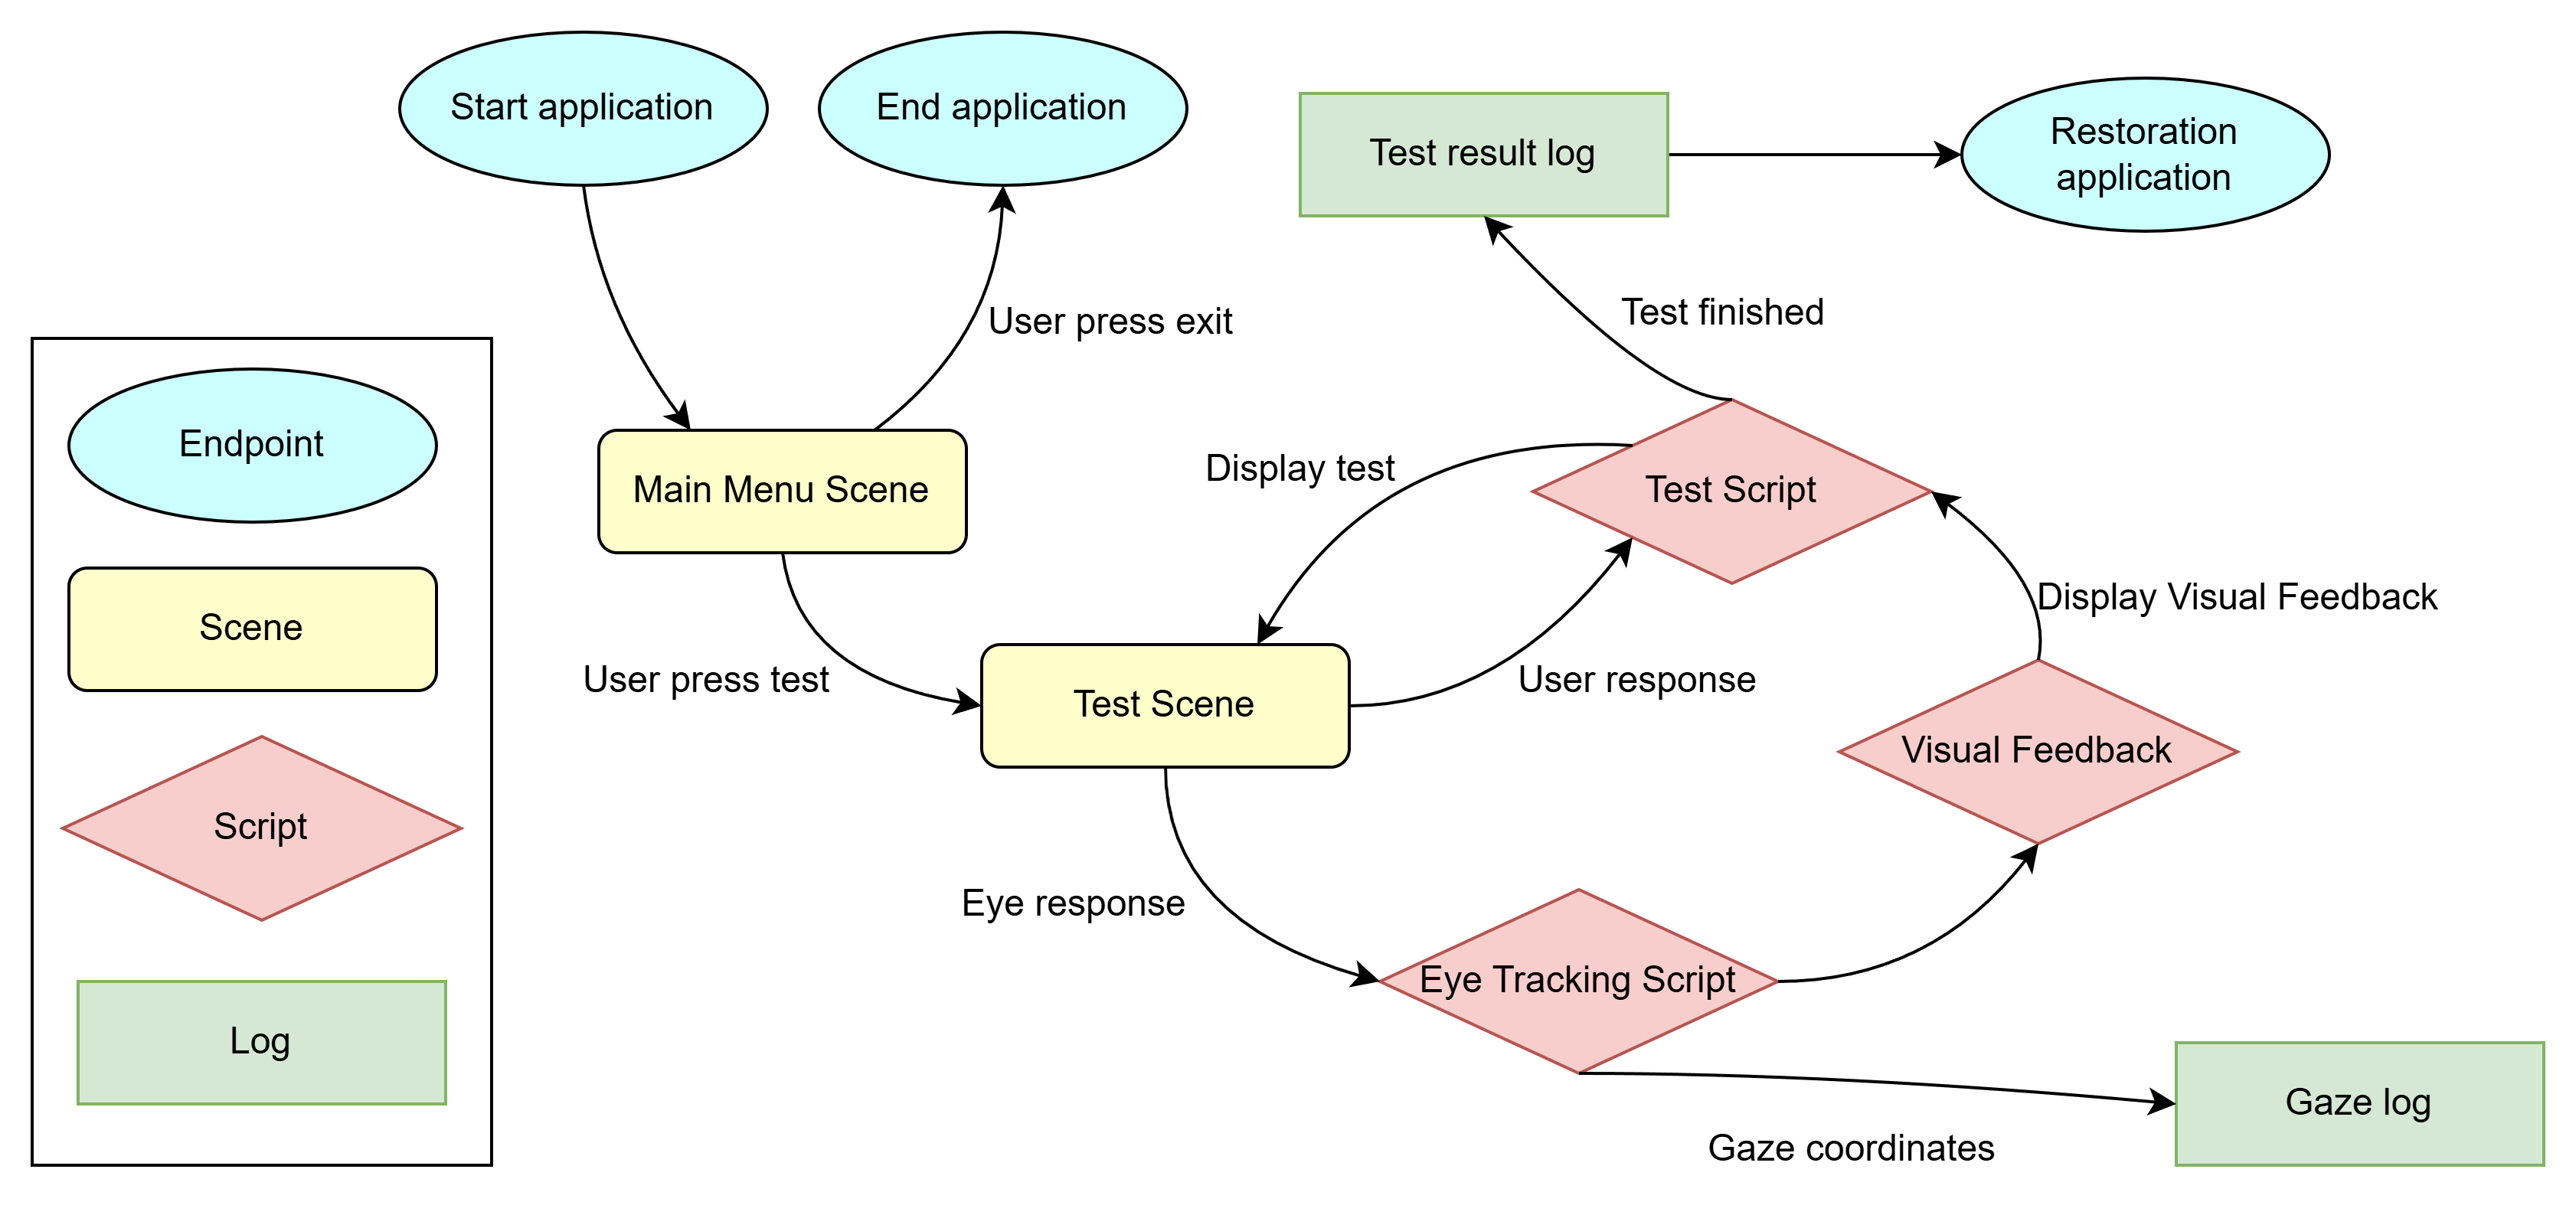
\includegraphics[width=1.0\linewidth]{images/High Level Diagram.png}
    \caption{A high-level diagram to show the design and workflow of the project}
    \label{fig: project workflow}
\end{figure}

\section{System Architecture}
The software is closely based on a Model-View-Controller software architecture pattern, following Unity’s scene and script-focused environment. This will help separate core functionalities to improve extensibility and maintainability.  

\subsection{Model}
The application uses serialisable data structures to record variables such as stimulus coordinates, detection responses, reaction times, and gaze fixation information. Serialisation into file formats like JSON allows for structured logging, easy data sharing, and downstream parsing and data processing using external tools such as Python. This design ensures that test results are both portable and readable. 

\subsection{View}
The view layer consists of Unity scenes rendered through a VR head-mounted display (HMD). This includes the main menu scene and the visual field testing scene. Users interact with the system by focusing on a fixation point and responding to the flashing stimuli. Real-time visual feedback is implemented to guide the user to focus on the fixation point, which will increase test reliability and user engagement. 

\subsection{Controller}
The Unity scripts act as the controllers. They handle all the logic of the system, like stimulus generation, gaze tracking, user input detection, and communication between different system components. The controllers also manage test flow and dynamically influence the view layer by calculating and providing visual feedback in real time. 

\section{User Interface and Input}

\subsection{User Interface}
The user interface is intentionally simple to ensure a focused testing experience. Interaction is driven primarily through gaze fixation and simple button press input. The interface is divided across two scenes: 

\begin{itemize}
    \item \textbf{Main Menu Scene:} \newline
         Presents the user with options to begin the test, read instructions, or exit the application. Future works may include adjustable settings such as different testing algorithms and grid density.

    \item \textbf{Visual Field Testing Scene:} \newline
        Displays a central fixation point and generates flashing stimulus dots in the peripheral field in front of a neutral colour and dim backdrop. Eye-tracking data is used to monitor whether the user maintains fixation.
\end{itemize}

\subsection{Input Handling}
User input is captured via keyboard or VR controller, depending on the deployment platform. The architecture is flexible enough to support future input modalities, such as electroretinography, in order to reduce user input errors.

\section{Workflow}  
The process is designed to simulate the logical flow of a clinical perimetry session while taking advantage of the interactive capabilities of virtual reality.

The workflow proceeds through the following stages, as shown in Figure \ref{fig: project workflow}: 

\begin{enumerate}
    \item \textbf{Session Initialisation:} \newline
        After turning on the headset, the user aligns the headset to ensure proper fit and comfort, and then begins the built-in eye-tracking calibration.

    \item \textbf{Main Menu:} \newline
        The user enters the main menu, where they can review brief instructions on how the test works and navigate to the visual test scene to begin the session.

    \item \textbf{Pre-Test Countdown:} \newline
         A short visual countdown is displayed to give the user time to focus on the central fixation point before the test begins.

    \item \textbf{Stimulus Generation:} \newline
        Visual stimuli are presented briefly at random positions within a defined radius around the central fixation point. A repeated fixed-intensity approach is used (see section \hyperref[sec: RFIA]{\textbf{4.3.1}}), where stimuli maintain the same brightness across the test but vary in positions, and each position or coordinate is tested multiple times.

    \item \textbf{Fixation Monitoring and Visual Feedback:} \newline
        Throughout the test, gaze monitoring is used to track whether the user maintains proper fixation, and gaze information is logged. Visual feedback could be activated, depending on the module, to help reinforce correct behaviour in real time for data reliability.

    \item \textbf{User Response Logging:} \newline
        For each stimulus, the user can indicate whether they detected it by pressing a button or trigger. Detection status and reaction times are logged for every test.

    \item \textbf{Test Completion and Data Finalisation:} \newline
        After all stimuli have been presented, the session ends automatically. All collected data is prepared for export, further analysis, and visualisation.
\end{enumerate}


\subsection{Repeated Fixed-Intensity Algorithm}
\label{sec:RFIA}
We developed a non-threshold visual field testing strategy that uses repeated presentations of a single, fixed-intensity stimulus at each test location. Unlike standard thresholding algorithms like SITA, this method does not attempt to determine the precise dimmest stimulus a participant can detect. Due to hardware limitations of being unable to calibrate the HMD’s absolute brightness, we instead employ a consistent brightness level across all stimuli and focus on participants’ detection consistency through multiple presentations.  

Specifically, for each point in the visual field, the stimulus is presented at the same location, in random order, a predefined number of times. The participant is asked to indicate whether they perceive each stimulus. The system then categorises the response based on how many times the participant reported seeing the stimulus. For example: 

\begin{itemize}
    \item \textbf{More than three detections}: the point is recorded as “consistently seen”

    \item \textbf{One or two detections}: the point is recorded as “inconsistently seen”

    \item \textbf{Zero detections}: the point is recorded as “unseen”
\end{itemize}

This design results in a simpler, more direct measurement of the visual field, at the cost of losing sensitivity data. Therefore, this repeated fixed-intensity approach can serve as a practical screening tool for a preliminary assessment before more extensive and sensitive threshold-based testing. 

\subsection{Data Storage}
The system is designed to collect and save user test data in a structured and portable format. To achieve this, all relevant data, such as stimulus locations, user responses, reaction times, and overall test duration, are stored in a data structure designed to support data collection and storage during runtime. 

Instead of writing data into the disk incrementally, the application maintains a data structure in memory that records all test-related information throughout the runtime. Once the test is completed, this data is serialised into a well-defined format (such as JSON) and saved to persistent storage. 

Each test run is saved into its own uniquely identified output folder to ensure traceability and to prevent overwriting or mixing data across sessions. This design supports later stages of the system, such as report generation, while also allowing for straightforward integration with external processing tools. 

\subsection{Report Generation}
Following test completion, a dedicated Python script can be executed to parse the saved data to generate a visual map of the user's visual field. This includes: 

\begin{itemize}
    \item A greyscale visual field map, showing which areas of the visual field were responsive

    \item A gaze detection density map, showing areas where the patient’s gaze was most frequently concentrated

    \item Metrics such as false positives and negatives, detection rate and average reaction time
\end{itemize}

The workflow of the report generation is shown in Figure \ref{fig: report workflow}.

The report may be exported as a PDF document, enabling easy sharing, printing, or clinical readings. The visual layout is inspired by conventional Humphrey Visual Field reports to aid interpretation and familiarity, as shown in Figure \ref{fig:hvf compare}.

\begin{figure}[!h]
    \centering
    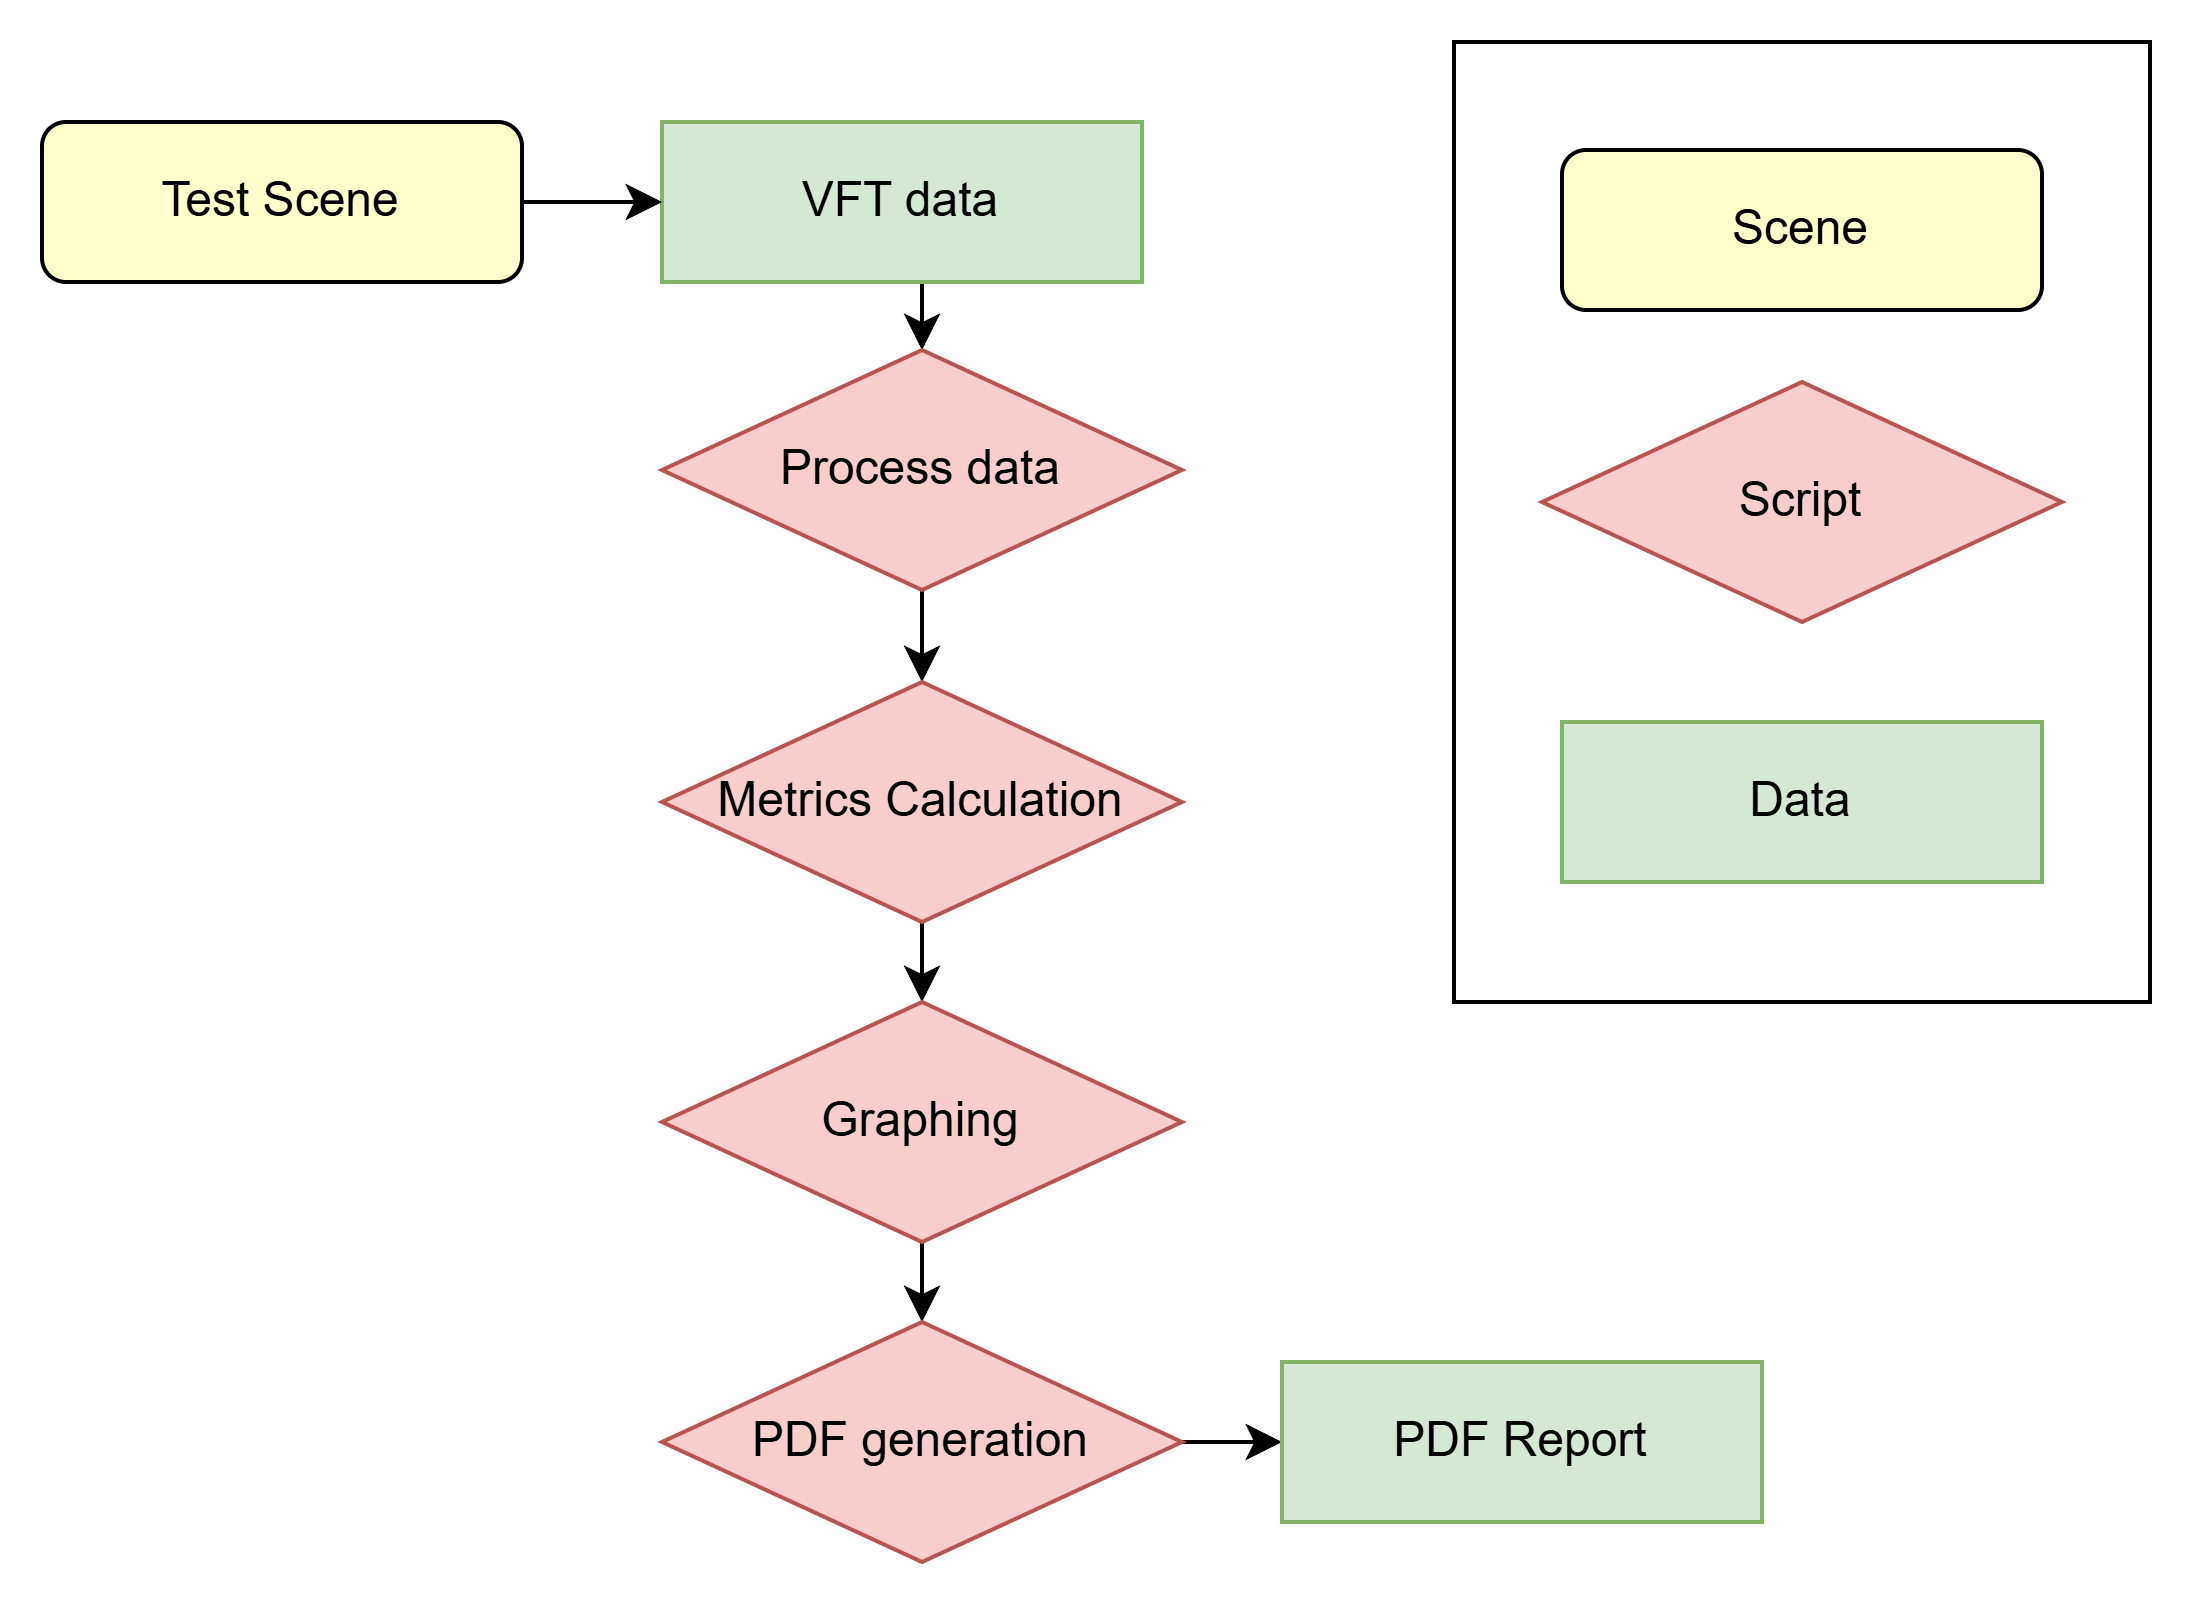
\includegraphics[width=0.75\linewidth]{images/Report Generation Workflow.png}
    \caption{A high-level diagram to show the workflow of the PDF report generation }
    \label{fig: report workflow}
\end{figure}



\section{Summary}

This chapter outlined the design of the VR-based visual field testing system, developed in response to the technical and usability requirements established in the previous chapter. The system follows an MVC architecture suited to Unity’s environment, promoting extensibility and maintainability.

The interface was designed to be minimal and intuitive, with gaze-based interaction and single-button input. The system includes a menu scene and a testing scene, with a workflow closely adapted from clinical perimetry procedures. A repeated fixed-intensity testing strategy was selected to accommodate hardware limitations while supporting satisfactory preliminary assessments.

Runtime data is stored in memory and serialised post-test, supporting structured export and further processing. A Python-based reporting workflow generates visual field maps and performance measures in a format that is similar to conventional clinical reports.

Together, these design decisions translated the identified requirements into a practical, extensible system. The next chapter will detail how this design was realised in implementation, covering the Unity environment, key scripts, object structures, and system integration with eye-tracking and data handling.

\begin{figure}[!h]
    \caption{}
    \label{fig:hvf compare}
    \centering
    \begin{subfigure}{.5\textwidth}
        \centering
        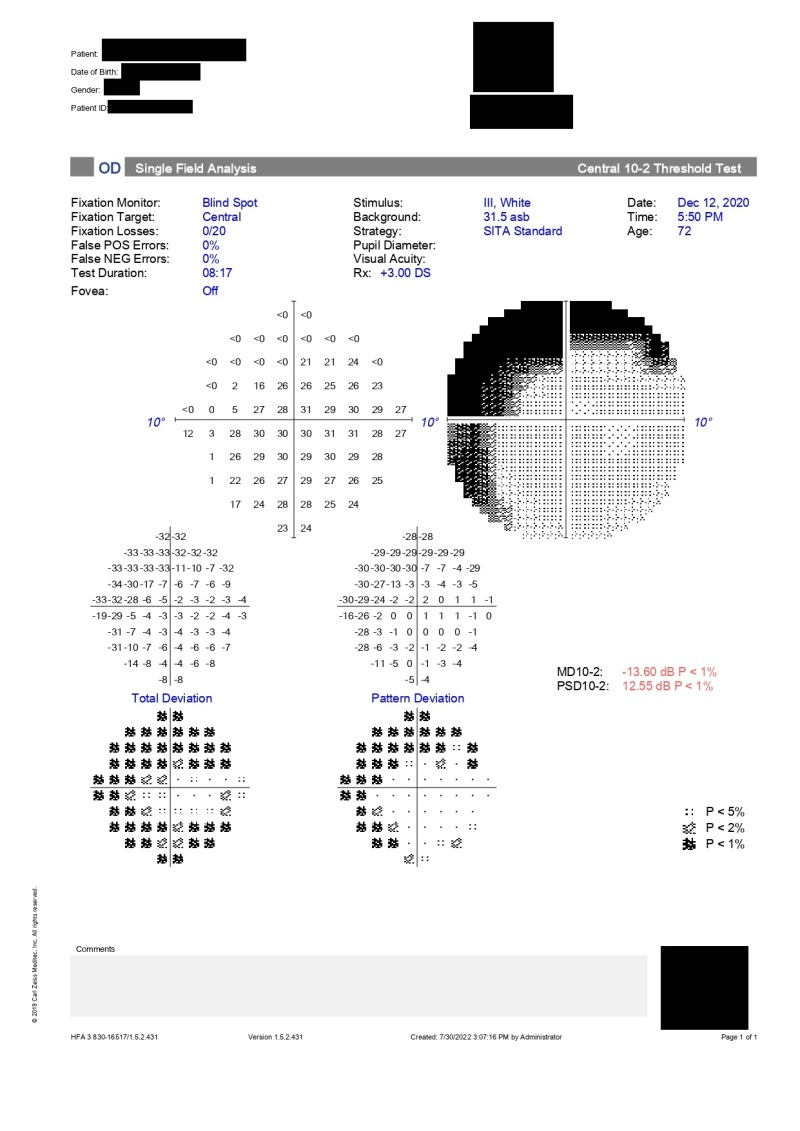
\includegraphics[width=1\linewidth]{images/ExampleofVFTreport.png}
        \vskip 0.5em
        \caption{Example of a standard HVF printout }
        \label{fig:standardHVFprint}
    \end{subfigure}%
    \begin{subfigure}{.5\textwidth}
        \centering
        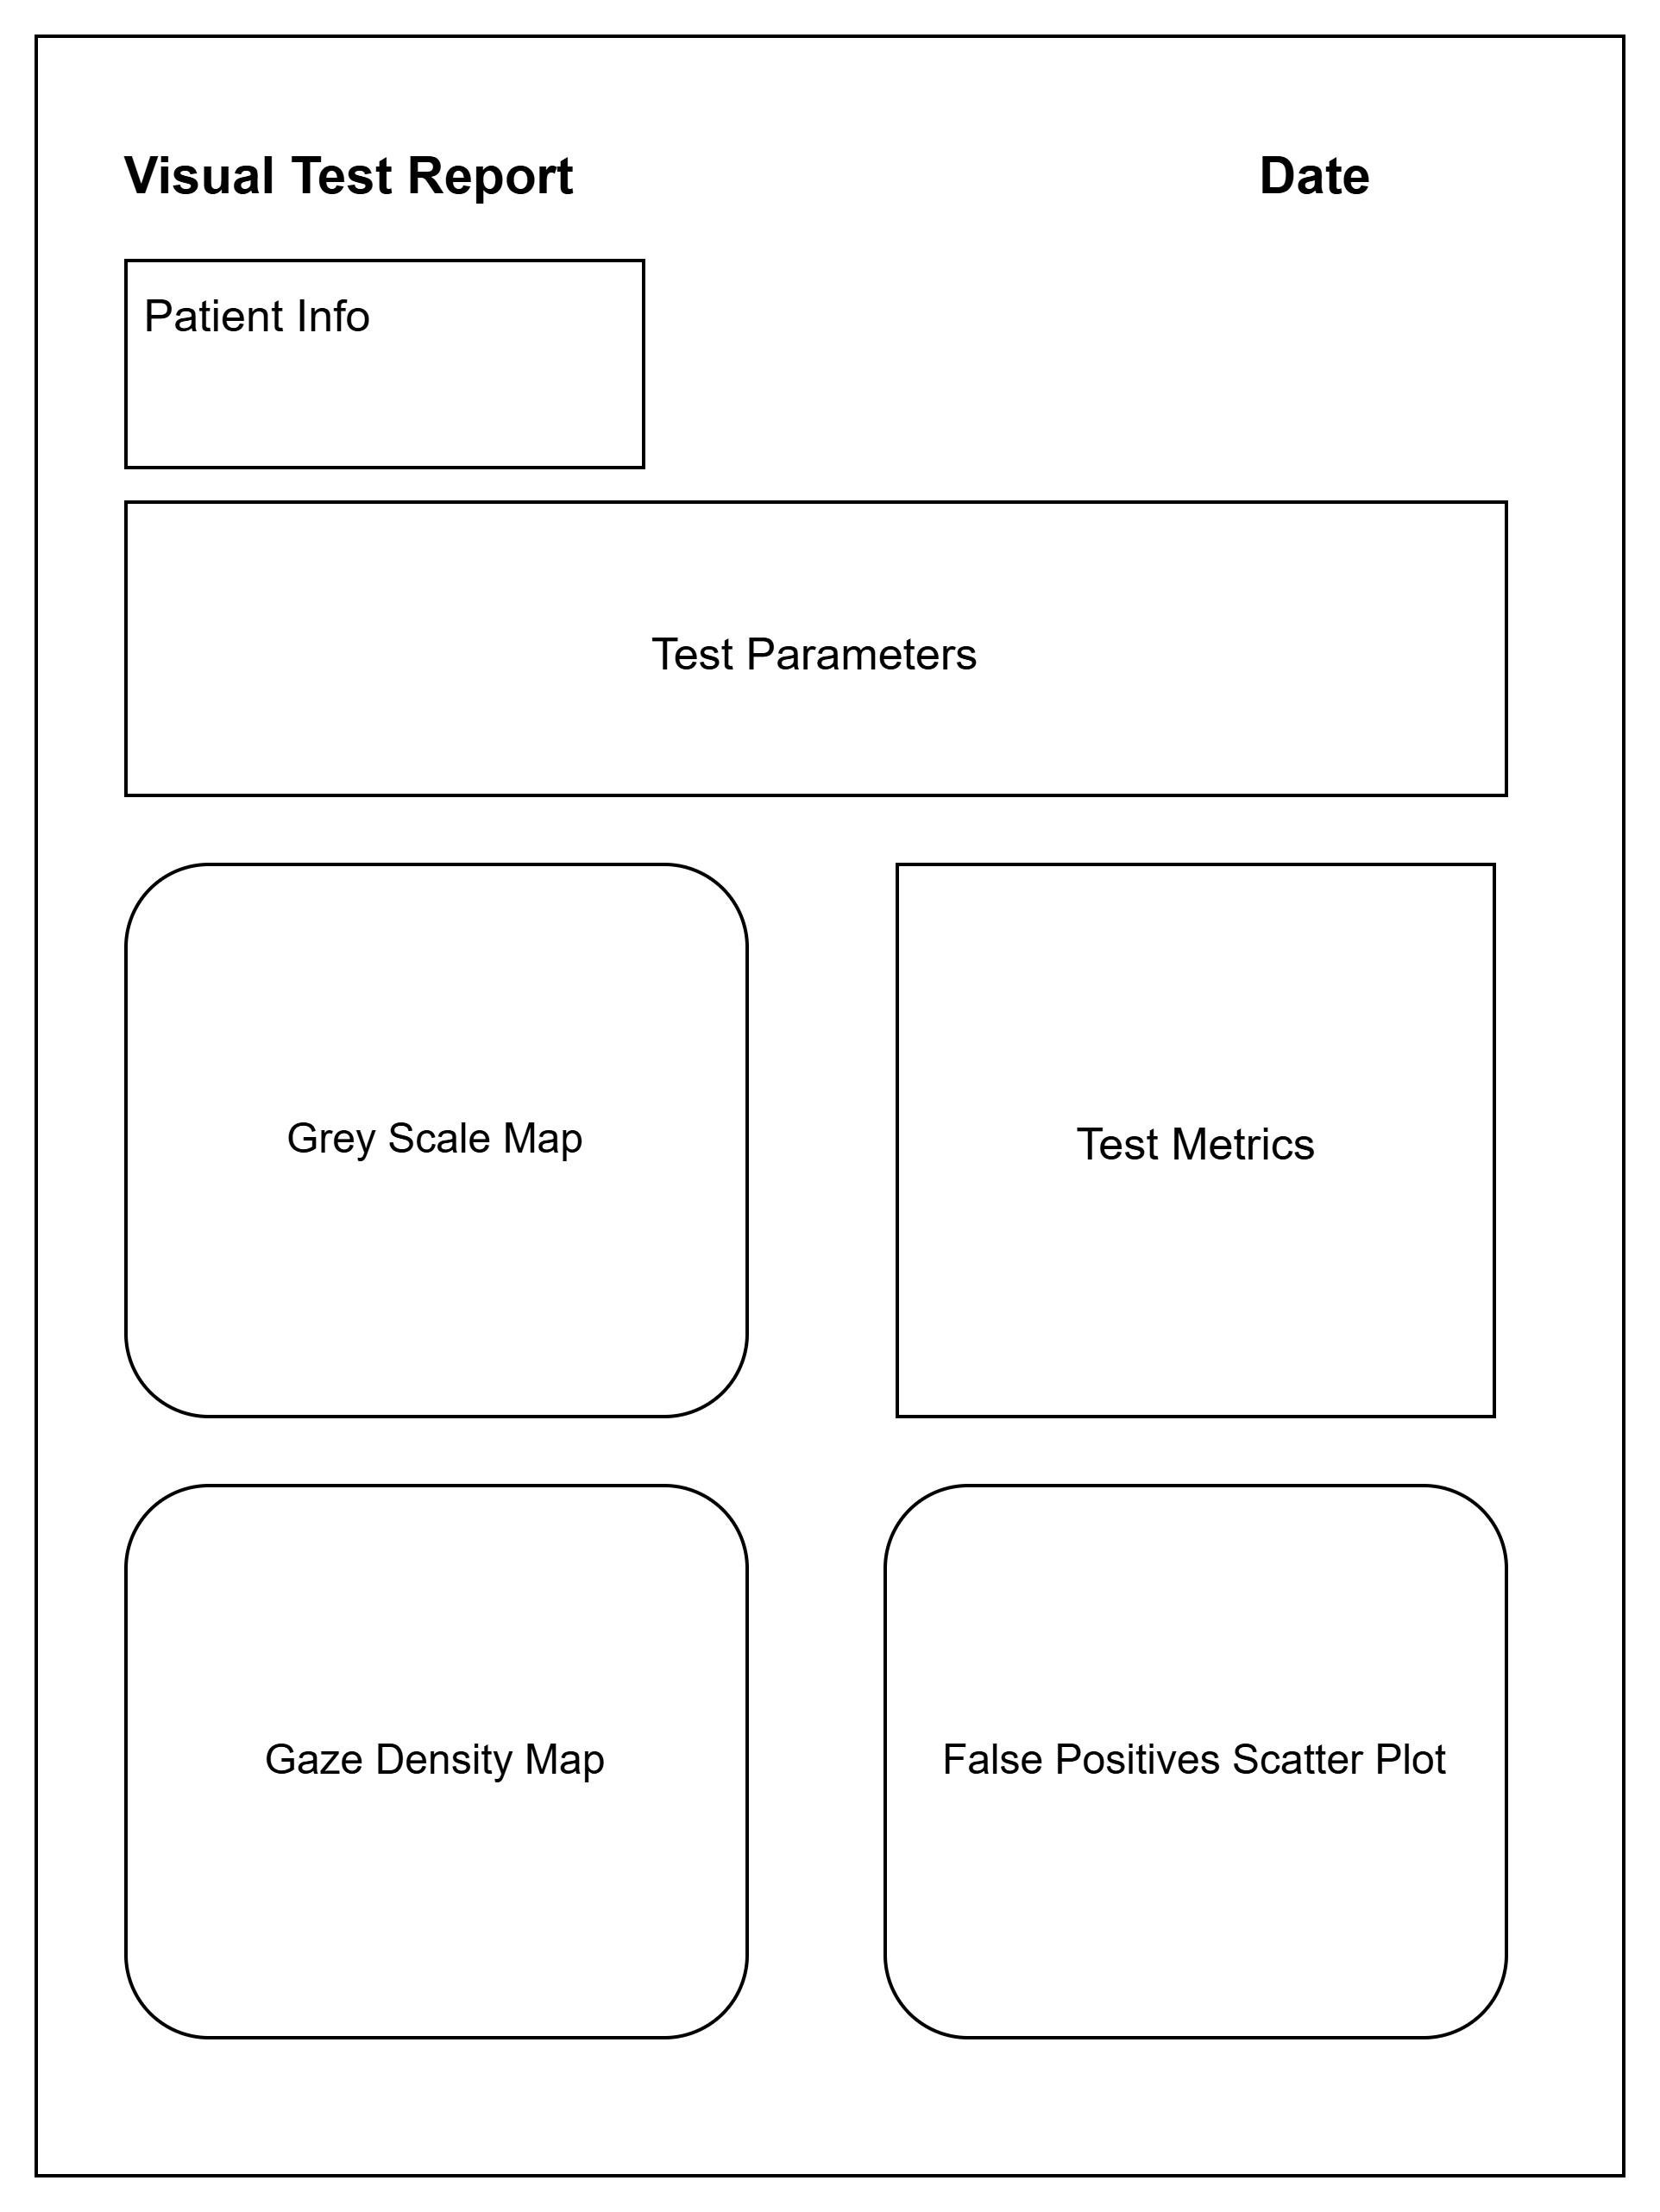
\includegraphics[width=1\linewidth,height=10cm]{images/Report Wireframe.png}
        \vskip 0.5em
        \caption{Wireframe of our PDF document}
        \label{fig:wireframeofPDF}
    \end{subfigure}%
\end{figure}

%==================================================================================================================================
\chapter{Implementation}

This chapter describes the practical implementation of the VR visual field testing system, following the designs outlined in the previous chapter. It outlines the hardware and software used, the structure of the Unity project, the core scripts developed, and the supporting user interface. All files are version-controlled using Git to support incremental development, collaboration, and secure backup.

The goal of this chapter is to show how each requirement was translated into working code, demonstrating the feasibility of delivering visual field testing through consumer-grade VR hardware.

\section{Development tools and Environment}
\subsection{UnityEngine}
The system was developed in Unity Editor 2019. Unity’s component-based architecture provides a flexible foundation for developing modular applications. We decided to use an older version of Unity Editor due to its support for SteamVR and its compatibility with the third-party SDK, SRanipal, for eye-tracking (see \ref{SDK}). This made it an appropriate choice for building a system requiring gaze-based interaction and stimulus control.

\subsection{Project Architecture}
As mentioned in the Design Chapter, the project adheres to a Model-View-Controller (MVC)-inspired architecture, where:
\begin{itemize}
    \item \textbf{Model:} Serialisable data structures store in-runtime data such as stimulus coordinates, gaze data, and response logs.

    \item \textbf{View:} Unity scenes represent the visual interface presented to the user.

    \item \textbf{Controller:} Scripts manage core logic, including stimulus generation, eye tracking, and data logging.
\end{itemize}

This structure, as shown in Figure \ref{fig:unityheir}, allows the separation of functionality and makes the system easier to debug, test, and extend. 

\begin{figure}[!h]
    \centering
    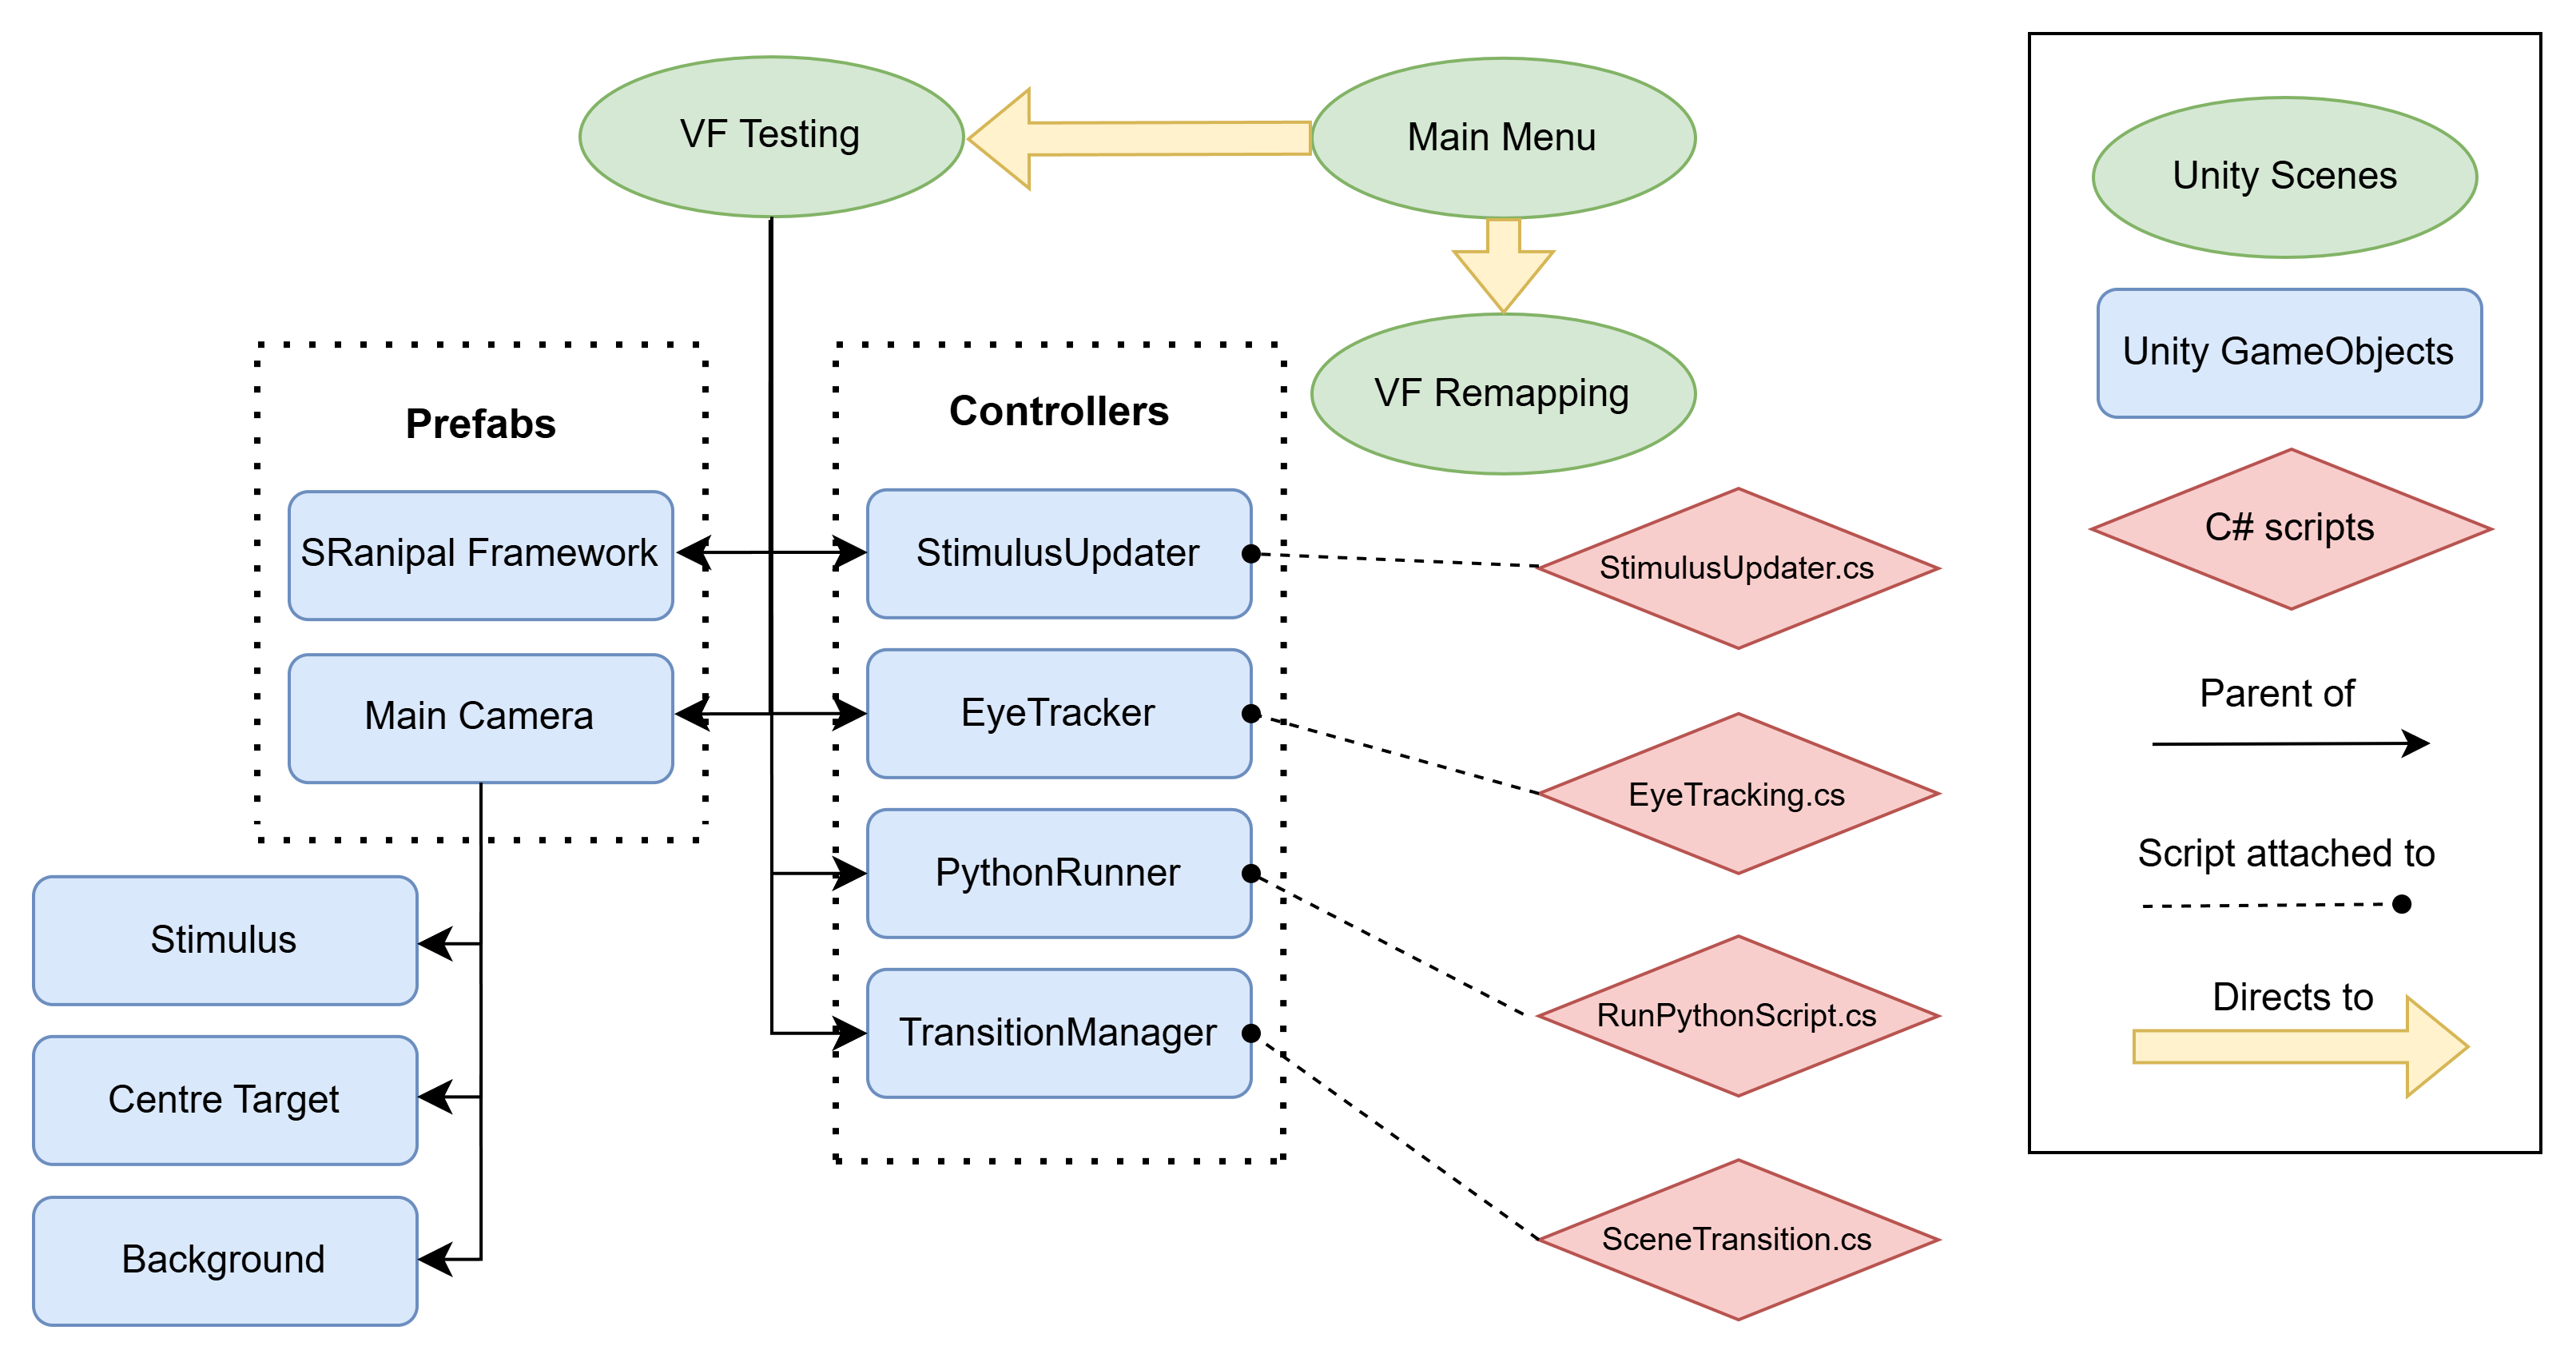
\includegraphics[width=1\linewidth]{images/Unity Heirarchy.png}
    \caption{shows an overview of the hierarchy of the Unity structure}
    \label{fig:unityheir}
\end{figure}

\section{Hardware Setup}

\subsection{Head-Mounted Display}
The application was developed for and tested on the HTC Vive Pro Eye, a SteamVR-compatible headset with integrated Tobii eye-tracking. The eye tracker enables real-time monitoring of gaze fixation, which is essential for accurate visual field testing. More details in \ref{hardware}.

\subsection{Workstation Specification}
Development and testing were performed on a workstation with the following specifications:

\begin{itemize}
    \item CPU: Intel Core i9-12900K
    
    \item GPU: NVIDIA RTX 3080 Ti

    \item RAM: 64 GB

    \item OS: Windows 11
\end{itemize}

These specifications are not strictly necessary but were used to ensure smooth VR performance and fast stimulus rendering, especially when running the application within the Unity Editor. Lower-spec hardware may result in frame drops or increased latency, which can interfere with accurate stimulus timing and user comfort.
 

\section{Scene and Object Structure}
\subsection{Unity Scenes}
The project is divided into two main scenes, shown in Figure \ref{fig:scenes}:

\begin{itemize}
    \item \textbf{MainMenu:} Provides the user with basic test instructions, start options, and, in future development, access to settings or alternative test modes.
 
    \item \textbf{VisualFieldTest:} Contains the full test environment where the stimuli are presented, gaze is monitored, and user responses are recorded.
\end{itemize}

\subsection{Core GameObjects}

Key GameObjects include:

\begin{itemize}
    \item \textbf{CenterDot:} A visual fixation sphere placed at the centre of the user’s field of view.
 
    \item \textbf{Stimulus:} A small sphere that is flashed at various positions to assess visual detection.
 
    \item \textbf{BackCanvas:} A neutral-coloured, dim background element providing contrast for the stimuli.
 
    \item Fixation Feedback: Uses colour changes to indicate gaze accuracy (e.g., green for focused, red for drift).
 
    \item \textbf{Managers:} GameObjects that coordinate stimulus generating, timing, eye-tracking, and data collection:
        \begin{itemize}
            \item StimulusUpdater
            \item EyeTracker
            \item PythonRunner
            \item Countdown
        \end{itemize}
    
\end{itemize}

Scripts are attached to Manager GameObjects to modularise behaviour and utilise Unity’s event lifecycle efficiently.

\section{Core Scripts and Functions}

\subsection{StimulusUpdater.cs}
Stimulus positions are defined within a bounded circular area surrounding the fixation point. A list of coordinates is generated at the start of the test and shuffled to randomise the stimulus sequence. Each position is tested multiple times in a repeated fixed-intensity algorithm.

\subsection{EyeTracking.cs}
Using the SRanipal SDK, eye position data is retrieved at runtime. The system checks whether the gaze falls within an acceptable angular range of the fixation point, by using a Ray GameObject that originates from the expected local coordinates of the user's gaze and checks whether it interacts with the colliders of the CenterDot. This fixation status is stored alongside the gaze coordinates and time data to enable visual feedback and post-analysis.

\subsection{Response Logging and Data Storage}
The system implements a custom serialisable class (saveData, marked [System.Serializable]) to handle runtime data collection and storage. During runtime, an instance of this class is created at the start of the test. As the test progresses, the user is asked to press the space key upon detection, and the application appends relevant data, such as stimulus positions, user detection status, and reaction time, directly into this instance. This allows the system to build a complete log of the session in memory, without writing to disk until the test is fully complete. When the test is completed, the full dataset is serialised using Unity’s built-in JsonUtility.ToJson() method. The resulting JSON string is then saved as a file within a uniquely named folder, timestamped to represent a single test run. This ensures that each session's data is isolated and traceable for later review and analysis. 

\section{Report Generation}
Post-test analysis is performed using a Python script triggered from within Unity. This script parses the JSON data and generates:

\begin{itemize}
    \item A greyscale visual field map showing detection reliability across coordinates.
 
    \item A gaze density map visualising where the user’s gaze was most concentrated.

    \item A scatter plot of the coordinates of the false-positive that the user logged. 
 
    \item Key performance metrics such as:
        \begin{itemize}
            \item Detection rate
         
            \item False positives
         
            \item Average reaction time
        \end{itemize}
\end{itemize}

The processed output is compiled into a PDF report, which emulates the style and layout of a Humphreys Visual Field (HVF) report for interpretability. This report is suitable for review by clinicians or researchers and supports consistent, session-by-session comparisons.

Figure \ref{fig:myVFTprintout} shows an example of the auto-generated VFT printout in PDF format.
In-depth explanation and code for the report generation in \ref{report generation}.

\begin{figure}[!h]
    \caption{}
    \centering
    \begin{subfigure}{.5\textwidth}
        \centering
        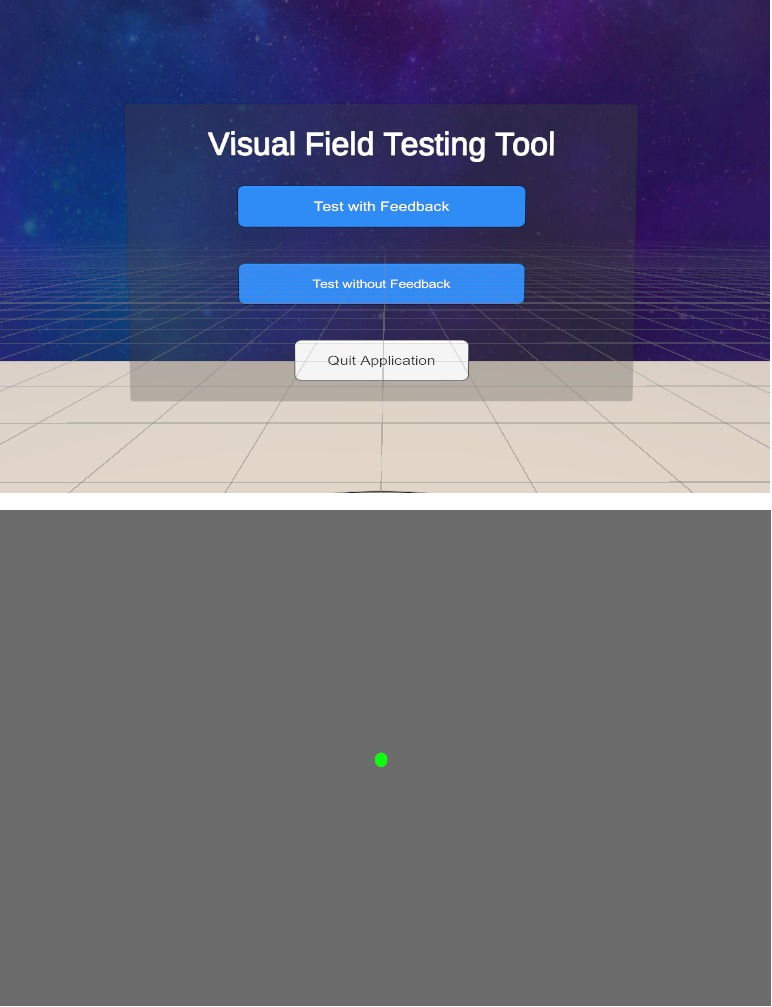
\includegraphics[width=1\linewidth,height=10cm]{images/Unity Scenes.jpeg}
        \vskip 0.5em
        \caption{Top shows the Main Menu Scene, Bottom shows the VFT scene }
        \label{fig:scenes}
    \end{subfigure}%
    \begin{subfigure}{.5\textwidth}
        \centering
        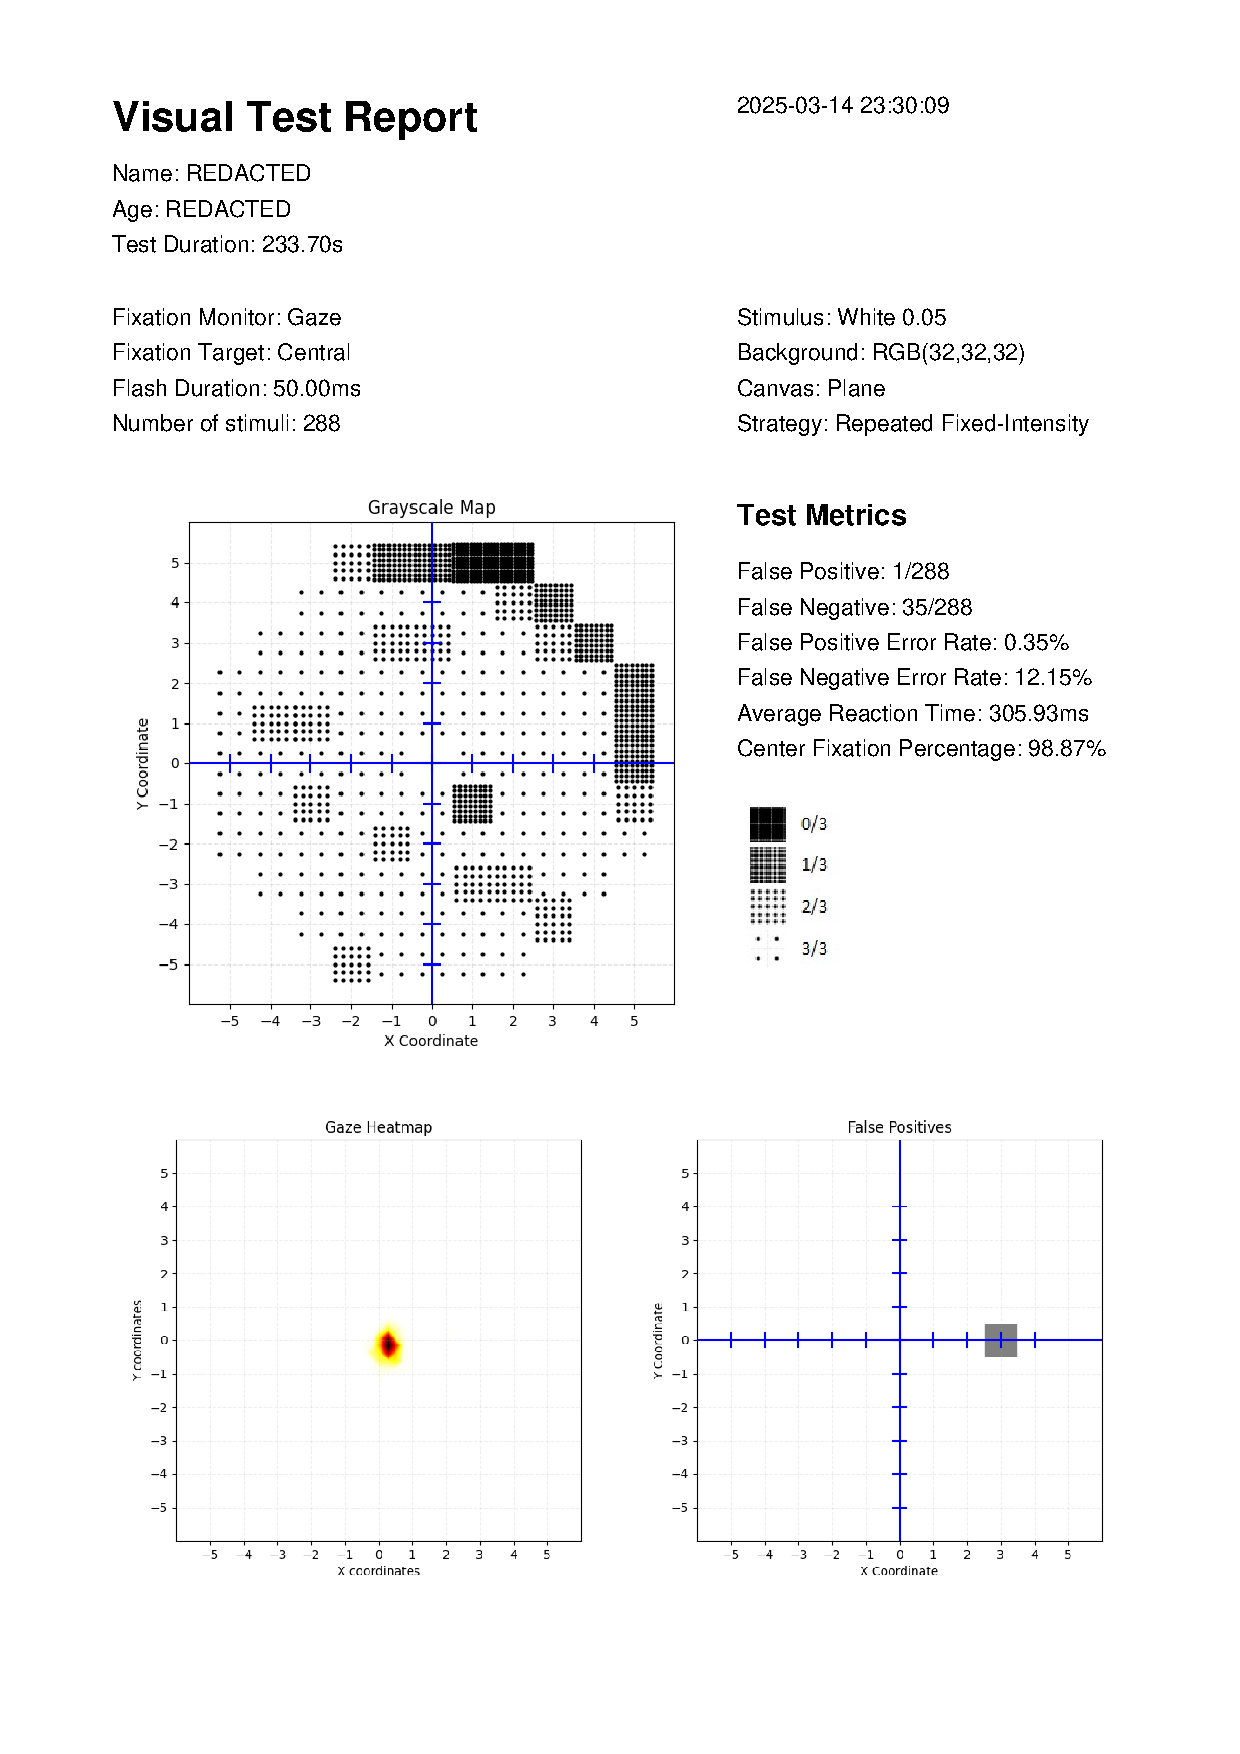
\includegraphics[width=1\linewidth]{images/Example of GVFT report.pdf}
        \vskip 0.5em
        \caption{Example generated VFT printout}
        \label{fig:myVFTprintout}
    \end{subfigure}%
\end{figure}

% \subsection{PDF scripts}
% \subsubsection{Data Parsing \& Processing}
% \subsubsection{Greyscale Figure Generation}
% \subsubsection{Gaze Density Figure Generation}
% \subsubsection{Metrics Calculations}
% \subsubsection{PDF Compilation}


\section{Summary}
This chapter details the implementation of the VR-based visual field testing system, covering software architecture, hardware setup, development environment, Unity scene design, and core scripts. The system uses a repeated fixed-intensity approach to accommodate hardware limitations, with user responses and eye-tracking data logged and analysed post-test. Outputs are processed into structured reports, supporting interpretation and future refinement. The modular Unity structure offers a flexible foundation for ongoing development and future adaptation.

In the next chapter, we evaluate the system’s effectiveness through informal feedback, pilot studies, and structured user testing. This includes both quantitative and qualitative measures, assessing usability, reliability, and the impact of design choices such as real-time fixation feedback.



%==================================================================================================================================
\chapter{Evaluation} 

This chapter presents the evaluation process for the VR-based visual field testing system. It outlines how informal observations and pilot studies influenced, explains the experimental setup and procedures, and reports the results of a small-scale user study. Both qualitative and quantitative measures were used to assess usability, user comfort, and the effects of real-time fixation visual feedback on user performance.

\section{Informal Observation}
Initial design evaluations were carried out through informal internal testing and iterative feedback discussions with the academic supervisor. These early observations highlighted that the repeated fixed-intensity testing approach offered significant implementation simplicity. However, it was also noted that this method sacrifices the ability to obtain finer sensitivity thresholds.

\section{Experiment Design}
Pilot studies were conducted to refine test parameters and assess user tolerability, leading to evidence-based decisions about stimulus design, test duration, and visual feedback. These studies, although exploratory, were essential in tailoring the system for novice users and aligning it with usability standards in VR and clinical physics. 

The following design parameters were refined through pilot studies, full details in \ref{sec:PilotStudiesDetails}:
\begin{itemize}
    \item Background Colour
    \item Eye Isolation
    \item Countdown Mechanism
    \item Stimulus Brightness and Size
    \item Reaction Time Allocation
    \item Testing Duration
    \item Rest Time Duration
\end{itemize}

\section{User Testing}
A small-scale user study was conducted to assess usability, comfort, and performance. The study used both subjective and objective measures, including the Simulator Sickness Questionnaire (SSQ) \citep{eval6}, the NASA Task Load Index (NASA-TLX) \cite{eval7}, and a custom evaluation questionnaire.

\subsection{Study Aims}
The primary question was whether real-time visual feedback would produce:
\begin{itemize}
    \item More accurate detection of peripheral stimuli (fewer negatives, faster reaction times).
    \item Reduced fixation losses (fewer false positives, higher centre fixation percentage).
\end{itemize}
Additional questions addressed comfort, simulator sickness, and perceived workload.

\subsection{Participants and Recruitment}
A total of 12 volunteers (age range 20-25) were recruited. All participants have limited exposure to VR and reported no known visual impairments. Participants provided consent and were free to withdraw at any time.


\subsection{Test Measures and Metrics}
\begin{itemize}
    \item \textbf{Simulator Sickness Questionnaire}: Administered post-test to assess symptoms like nausea, eye strain, and disorientation.
    \item \textbf{NASA Task Load Index}: Evaluated perceived workload in terms of factors such as mental, physical, temporal, effort, performance, and frustration.
    \item \textbf{Custom Evaluation Questionnaire}: Gathered qualitative feedback about comfort, ease of use, and further development ideas. 
    \item \textbf{Objective Test Metrics}:
        \begin{itemize}
            \item \textbf{Center Fixation Percentage:} How often participants maintained fixation on the designated centre point.
            
            \item \textbf{Reaction Time (RT):} Measured as time from stimulus onset to button press.

            \item \textbf{False Positive (FP) rate:} False positives occur when the participant presses the response button even when they were not properly fixating on the centre target.
            
            \item \textbf{Negative (N) rate:} Negatives occur when the participant fails to respond to a stimulus that was in fact displayed.
            
        \end{itemize}
\end{itemize}



\subsection{Study Procedure}
\begin{enumerate}
    \item \textbf{Briefing and Calibration:} After a brief introduction, participants were familiarised with the VR headset and underwent eye-tracker calibration.
    \item \textbf{Counterbalancing:} A partial Latin square design was used to alternate the order of conditions to reduce learning effect and order biases. Each eye (left or right) and each feedback mode (with or without visual feedback) was tested.
    \item \textbf{Testing Conditions:} 
        \begin{itemize}
            \item \textbf{Condition A (Without Real-Time Visual Feedback)} The central fixation point stayed green for the entire test duration.
            \item \textbf{Condition B (With Real-Time Visual Feedback)} The central fixation point would indicate whether the participant was fixating on the central target. 
        \end{itemize}
    \item \textbf{Data Collection:} For each condition, the system recorded reaction times, detection success or failure, and gaze tracking data. Participants also completed an SSQ form after each condition.
    \item \textbf{Rest Periods:} Participants removed the headset between conditions and were allowed to rest to minimise discomfort and simulator sickness.
\end{enumerate}


\section{Quantitative Data Analysis}
All quantitative analyses were performed using paired \emph{t}-tests (within-subjects design). For each participant, we compared Condition~A (no feedback) versus Condition~B (with feedback):
\begin{itemize}
    \item \textbf{\emph{Null Hypothesis} $(H_0)$}: There is no difference in performance metrics between the two conditions.
    \item \textbf{\emph{Alternative Hypothesis} $(H_a)$}: There is a difference between the two conditions (two-sided test).
\end{itemize}
Statistical significance was assessed at $\alpha=0.05$. Effect sizes (Cohen's $d$) were also calculated to estimate the magnitude of any significant effects.

\subsection{Center Fixation Percentage} 

When participants had real‐time fixation feedback, we expected them to maintain centre gaze more consistently. For most participants, centre fixation percentage was indeed higher in the feedback condition. However, with all 12 data sets included, the difference in centre fixation percentage approached but was not statistically significant ($p \approx 0.071 > 0.05$) (as shown in Table \ref{tab:CF}).

This is due to an outlier, Participant 8. During the user study, Participant 8 was noted to have difficulties focusing on the test and was distracted on multiple occasions. Therefore, Participant 8 was removed from all further statistical analyses.

Upon removing Participant 8, whose data indicated extremely erratic fixation, the difference became statistically significant ($p \approx 0.017 < 0.05$), and $d \approx 0.87$, suggesting a relatively large effect of visual feedback on centre fixation, as shown in Table \ref{tab:CFno8}. 


These results allow us to reject the null hypothesis for centre fixation percentage after removing the outlier (Participant 8), supporting the alternative hypothesis that real-time feedback improves centre fixation consistency.

 We present both versions to illustrate how a single participant’s data can influence statistical outcomes.

\begin{table}[!h]
    \centering
    \renewcommand{\arraystretch}{1.5}
    \begin{tabular}{|c|c|c|c|c|c|c|c|}
        \hline
        Test Condition & $CF$ \% & $m_D$ & $s_d$  & $SEM$ & $t$ & $p$ & $d$  \\
        \hline
        Without Feedback & 62.88 \% & \multirow{2}{*}{11.42 \%} & \multirow{2}{*}{19.80 \%} & \multirow{2}{*}{5.72 \%} & \multirow{2}{*}{2.00} & \multirow{2}{*}{0.071} & \multirow{2}{*}{0.58}\\ \cline{1-2}
 
        With Feedback & 74.30 \% & {} & {} & {} & {} & {} & {}\\ 
    
        \hline
    \end{tabular}
    \vskip 0.5em
    \caption{Center fixation percentage ($CF$ \%) without feedback vs. with feedback, showing mean difference ($m_D$), standard deviation ($s_D$), standard error ($SEM$), t‐statistic ($t$), p‐value ($p$), and effect size ($d$).}
    \label{tab:CF}
\end{table}

\begin{table}[!h]
    \centering
    \renewcommand{\arraystretch}{1.5}
    \begin{tabular}{|c|c|c|c|c|c|c|c|}
        \hline
        Test Condition & $CF$ \% & $m_D$ & $s_d$  & $SEM$ & $t$ & $p$ & $d$  \\
        \hline
        Without Feedback & 60.31 \% & \multirow{2}{*}{14.71 \%} & \multirow{2}{*}{16.98 \%} & \multirow{2}{*}{5.12 \%} & \multirow{2}{*}{2.87} & \multirow{2}{*}{0.017} & \multirow{2}{*}{0.87}\\ \cline{1-2}
 
        With Feedback & 75.01 \% & {} & {} & {} & {} & {} & {}\\ 
  
        \hline
    \end{tabular}
    \vskip 0.5em
    \caption{Center fixation percentage without feedback vs. with feedback, without Participant 8}
    \label{tab:CFno8}
\end{table}

\subsection{Response Time} 

We initially hypothesised that visual feedback might help participants respond faster to stimuli. However, the results showed that participants actually responded more slowly when feedback was provided.

\begin{table}[!h]
    \centering
    \renewcommand{\arraystretch}{1.5}
    \begin{tabular}{|c|c|c|c|c|c|c|c|}
        \hline
        Test Condition & $RT$ (ms) & $m_D$ & $s_d$  & $SEM$ & $t$ & $p$ & $d$  \\
        \hline
        Without Feedback & 306.31 ms & \multirow{2}{*}{12.28 ms} & \multirow{2}{*}{14.39 ms} & \multirow{2}{*}{4.34 ms} & \multirow{2}{*}{2.83} & \multirow{2}{*}{0.018} & \multirow{2}{*}{0.85}\\ \cline{1-2}
     
        With Feedback & 318.59 ms & {} & {} & {} & {} & {} & {}\\ 
    
        \hline
    \end{tabular}
    \vskip 0.5em
    \caption{Response Time ($RT$) without feedback vs. with feedback, showing mean difference ($m_D$), standard deviation ($s_D$), standard error ($SEM$), t‐statistic ($t$), p‐value ($p$), and effect size ($d$).}
    \label{tab:RT}
\end{table}

Since the mean difference is positive, participants took approximately 12 ms longer to respond with feedback. This result (shown in Table \ref{tab:RT}) was statistically significant ($p \approx 0.018$), and $d \approx 0.85$ suggests a relatively large effect. With this, we can reject the null hypothesis and accept the alternative that feedback affects reaction time. However, the direction of this effect was contrary to the initial expectation. Feedback led to slower responses rather than faster responses.


Possible Reasons for Slower Reaction Time with Feedback:
\begin{itemize}
    \item \textbf{Heightened Caution:} Participants might have slowed their responses in order to verify that they were properly fixating before pressing the button.
    \item \textbf{Increased cognitive load:} Having the centre target changing colours adds a visual element that might slightly divide attention or increase decision time.
\end{itemize}


\subsection{False Positive Error Rate}

\begin{table}[!h]
    \centering
    \renewcommand{\arraystretch}{1.5}
    \begin{tabular}{|c|c|c|c|c|c|c|c|}
        \hline
        Test Condition & $FP$ \% & $m_D$ & $s_d$  & $SEM$ & $t$ & $p$ & $d$  \\
        \hline
        Without Feedback & 16.87 \% & \multirow{2}{*}{-12.19 \%} & \multirow{2}{*}{13.86 \%} & \multirow{2}{*}{4.18 \%} & \multirow{2}{*}{-2.92} & \multirow{2}{*}{0.015} & \multirow{2}{*}{0.88}\\ \cline{1-2}

        With Feedback & 4.69 \% & {} & {} & {} & {} & {} & {}\\ 
        \hline
    \end{tabular}
    \vskip 0.5em
    \caption{False positive error rate ($FP$ \%) without feedback vs. with feedback, showing mean difference ($m_D$), standard deviation ($s_D$), standard error ($SEM$), t‐statistic ($t$), p‐value ($p$), and effect size ($d$).}
    \label{tab:FP}
\end{table}

When participants had visual feedback, we hypothesised that they would press the response button only if they were properly fixating on the centre target, thus reducing false positives. Among 11 participants, the mean difference (as shown in Table \ref{tab:FP}) was -12.19\%, $p \approx 0.015$, and $d \approx 0.88$ suggest statistical significance and a moderately large effect size, and the negative sign indicates that visual feedback helps reduce unfocused button presses. We can reject the null hypothesis and conclude that feedback significantly reduces false positive errors. This supports the idea that participants respond more accurately when guided by real-time gaze feedback.

\newpage
\subsection{Negative Error Rate}


Somewhat unexpectedly, negative rate actually increased under real‐time feedback for several participants. However, as seen in Table \ref{tab:FN}, the difference was not statistically significant ($p \approx 0.124 > 0.05$) and had only a medium effect size ($d \approx 0.43$). In other words, participants with feedback sometimes missed more stimuli compared to when they had no feedback. \newline

Possible Reasons for More Misses:
\begin{itemize}
    \item \textbf{Visual Distraction:} The feedback may have drawn participants’ attention towards the centre, causing them to overlook some peripheral stimuli.
    \item \textbf{Tunnel Vision:} Participants may have focused too rigidly on maintaining fixation, making them less responsive to new peripheral flashes.
\end{itemize}

\begin{table}[!h]
    \centering
    \renewcommand{\arraystretch}{1.5}
    \begin{tabular}{|c|c|c|c|c|c|c|c|}
        \hline
        Test Condition & $N$ \% & $m_D$ & $s_d$  & $SEM$ & $t$ & $p$ & $d$  \\
        \hline
        Without Feedback & 15.25 \% & \multirow{2}{*}{2.29 \%} & \multirow{2}{*}{5.35 \%} & \multirow{2}{*}{1.61 \%} & \multirow{2}{*}{1.42} & \multirow{2}{*}{0.19} & \multirow{2}{*}{0.43}\\ \cline{1-2}
        With Feedback & 17.54 \% & {} & {} & {} & {} & {} & {}\\ 
       
        \hline
    \end{tabular}
    \vskip 0.5em
    \caption{Negative error rate ($FN$ \%) without feedback vs. with feedback, showing mean difference ($m_D$), standard deviation ($s_D$), standard error ($SEM$), t‐statistic ($t$), p‐value ($p$), and effect size ($d$).}
    \label{tab:FN}
\end{table}

As the results are not statistically significant, we fail to reject the null hypothesis for negative rates. There is no strong evidence that feedback had a significant effect on missed stimuli. Further studies with larger samples would be needed to determine whether the trend is a real phenomenon or simply noise.


\section{Subjective Measures}

\subsection{Simulator Sickness and Comfort} 

Participants rated the comfort of the VR headset on a scale from 1 (Very Uncomfortable) to 5 (Very Comfortable). The average rating was 4, with the majority of users (10 out of 12) reporting the headset as either "comfortable" or "very comfortable." This suggests that the physical hardware setup was generally well-received, and short-duration test sessions did not result in notable discomfort from the headset itself.

Symptom severity ratings were captured on a 5-point scale ranging from “None” (1) to “Always” (5), as shown in Figure \ref{fig:ssqbar}. The most commonly reported symptoms were eye strain (mean $\approx$ 3.0) and fatigue (mean $\approx$ 2.6), followed by difficulty focusing and general discomfort, both in the moderate range. These symptoms are consistent with the demands of maintaining fixation and responding to stimuli in a visually focused task. However, symptoms often associated with simulator sickness, such as nausea, blurred vision, and headache, were rated relatively low, with nausea being the least reported.

These findings suggest that while the task did impose some visual and cognitive load, the system design successfully minimised discomfort traditionally associated with VR environments. The neutral grey background, short trial durations (4–5 minutes), and provided rest breaks appear to have effectively reduced symptoms of simulator sickness.

Overall, the system was perceived as comfortable and tolerable, with no participants needing to discontinue due to sickness or discomfort.

\begin{figure}[!h]
    \centering
    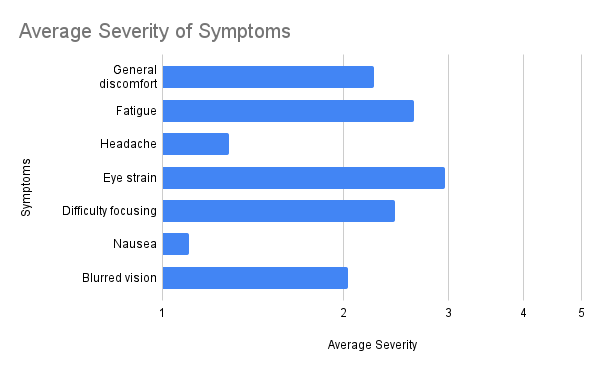
\includegraphics[width=0.75\linewidth]{images/SSQ barchart.png}
    \caption{Average severity of symptoms of Simulator Sickness}
    \label{fig:ssqbar}
\end{figure}

\newpage

\subsection{NASA-TLX} 
To assess participants' perceived workload during the test sessions, a simplified version of the NASA Task Load Index (NASA-TLX) was administered at the end of the study. Participants rated six workload-related factor using a 5-point scale ranging from 1 (Very Low) to 5 (Very High):

\begin{itemize}
    \item Mental demand
    \item Physical demand
    \item Temporal demand (hurried or rushed pace)
    \item Performance (perceived success)
    \item Effort (how hard they had to work)
    \item Frustration (insecurity, stress, annoyance)
\end{itemize}

Each factor was scored independently. The average ratings across all participants were shown in Figure \ref{fig:nasabar}.

Result interpretation:
\begin{itemize}
    \item Mental demand received low-to-moderate scores (mean $\approx$ 2.75), suggesting that the task requires visual attention and quick responses, but not overly complex or mentally taxing.
    \item Physical demand received a surprisingly moderate score (mean $\approx$ 3.08), which may reflect the repeated key presses and the need to maintain posture during trials.
    \item Temporal demand was also moderate (mean $\approx$ 2.67), indicating that participants generally felt the pace was manageable and not excessively rushed.
    \item Participants felt highly successful in completing the task (mean $\approx$ 4.00), and simultaneously reported putting in a relatively high level of effort (mean $\approx$ 4.08). This suggests that while the test required concentration and engagement, users remained confident and committed to the task.
    \item Frustration levels were moderate (mean $\approx$ 2.50), suggesting some differences in how comfortable or emotionally relaxed participants felt, though no overwhelming stress was reported.
\end{itemize}

Overall, the task was perceived as moderately demanding and effortful, but not overwhelming. Users felt successful and mostly not overly frustrated by the experience. These findings support the suitability of the test for short-term use in a VR setting.

\newpage

\begin{figure}[!h]
    \centering
    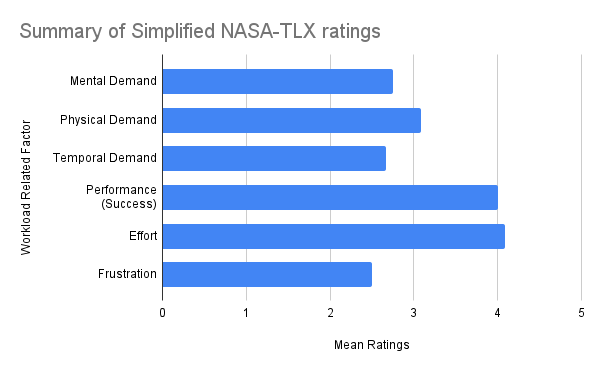
\includegraphics[width=0.75\linewidth]{images/NASATLX barchart.png}
    \caption{Summary of simplified NASA-TLX ratings of each workload-related factors}
    \label{fig:nasabar}
\end{figure}



\section{Qualitative Feedback}
The evaluation questionnaire provided additional insights from the participants:
\begin{itemize}
    \item \textbf{Clarity of instructions:} All of the participants found the instructions given to be very clear. 
    \item \textbf{Difficulty Focusing:} A third of the participants found it easy to focus on the centre target, half of them remained neutral, and the remaining two participants found it difficult to focus on the centre target throughout the test.
    \item \textbf{Usefulness of Visual Feedback:} 75\% of the participants found the visual feedback helpful, stating it helped them focus and guided them to maintain a stable gaze. The other 25\% of the participants considered it an unnecessary distraction, suggesting that experienced users might prefer minimal on-screen cues.
    \item \textbf{User experience:} The majority of the participants found the concept to be interesting and fun, with 41.6\% of the participants also finding it tiring.
\end{itemize}

\section{Limitations}
\begin{itemize}
    \item \textbf{Outliers and Small Sample Size:} With only $n=12$ participants, a single outlier could heavily influence results, as shown by the performance of Participant 8. Future larger-scale studies would result in greater statistical significance.
    \item \textbf{Fatigue and Attention Effects:} Despite given breaks, some participants chose not to fully utilise the full rest period and wanted to proceed earlier. Some participants also displayed inattentive behaviour, such as random or rhythmic button pressing, near the end of testing.
    \item \textbf{Hardware and Environmental Constraints:} Device-level factors such as inconsistent eye-tracker calibration, slight headset misalignments, or fluctuations in screen brightness may have introduced additional unaccounted factors between participants. These technical inconsistencies are difficult to control in a typical lab setting but can meaningfully affect stimulus perception.
\end{itemize}

\section{Summary}

This chapter evaluated the performance and user experience of the VR-based visual field testing system through both quantitative and qualitative measures. Objective metrics indicated that real-time fixation feedback improved centre fixation consistency and reduced false positive responses, although it also resulted in slightly slower reaction times. Negative rates showed a small, non-significant increase when feedback was enabled. The impact of outliers, particularly Participant 8, was notable in some cases and demonstrates the need for a larger-scale user study to reduce user variance. 

Subjective responses generally reflected a positive user experience. Most participants rated the headset as comfortable and tolerated the testing procedure well. While symptoms such as eye strain and fatigue were commonly reported, their severity remained moderate. NASA-TLX ratings showed that participants felt they had to exert effort and concentration, but still perceived themselves as successful in completing the task, with low levels of frustration overall.

Overall, the results support the feasibility of the system for short-term diagnostic use in VR. However, they also highlight areas for refinement, such as visual comfort, task pacing, and broader user testing with a larger participant pool. The next chapter provides a final reflection on the project, revisiting its objectives and results, and outlining directions for future development.


%==================================================================================================================================

\chapter{Conclusion}    


\section{Summary}

This dissertation has presented the design, development, and evaluation of a VR-based visual field testing system, using consumer-grade virtual reality hardware with integrated eye-tracking. The system was designed to offer a more accessible and cost-effective alternative to traditional perimetry devices, such as the Humphrey Visual Field Analyser, which is mostly confined to clinical settings due to its large size, high cost, and supervision requirements. 

The project followed a structured design and implementation process, guided by the Model-View-Controller design pattern within Unity’s component-based architecture. The software incorporated a simple user interface, stimulus generation algorithms, real-time fixation visual feedback mechanisms, and structured data logging, and integrated them into a coherent visual testing environment. Stimuli were presented at fixed intensity using a repeated fixed-intensity strategy, simplifying the overall testing process while still enabling meaningful evaluation of visual field performance. 

A key feature of the system is its use of eye-tracking for real-time fixation monitoring, which not only improves test reliability but also helps guide the user during the test. This feedback system proved to be particularly useful during preliminary evaluations, where users demonstrated improved focus and reduced response error when visual feedback was enabled. 

Through pilot studies and a user study (n = 12), the system’s core functionality and user experience were iteratively refined. The pilot study helped inform decisions on design parameters such as stimulus flash duration, background colour, response time window, and test duration. 

Quantitative data analysis showed that having visual feedback significantly improved certain performance metrics. After removing one notable outlier, centre fixation percentage improved by an average of 14.71\% with visual feedback enabled ($p = 0.017$, $d = 0.87$). False positive rates also decreased by an average of 12.19\% ($p = 0.015$, $d = 0.88$), suggesting users responded more cautiously and accurately. However, reaction times were, on average, 12.28 ms slower in the feedback condition ($p = 0.018$, $d = 0.85$), potentially indicating increased cognitive load or divided attention. Negative rates increased slightly with feedback but did not reach statistical significance ($p = 0.19$), leaving the effect inconclusive.

Subjective feedback via the Simulator Sickness Questionnaire (SSQ) and NASA Task Load Index (NASA-TLX) indicated that the system was generally well-tolerated. Users reported moderate levels of eye strain and fatigue, but low levels of nausea or frustration. Most participants rated the headset as comfortable and felt successful in completing the test.

While the results are not yet generalisable to clinical use, the system demonstrates the feasibility of using VR as a platform for preliminary visual field screening, especially in non-clinical or remote settings. The modular and extensible nature of the system also makes it possible for future enhancements and possible clinical integration. 

\section{Reflection}
Early in development, I underestimated the complexity of implementing eye-tracking in Unity, particularly due to the SRanipal SDK no longer being supported. Getting stable eye-tracking data required more effort than expected. Through repeated iteration and pilot testing, I gained a much deeper understanding of system calibration, user testing protocols, and how small interface changes could significantly affect user performance and comfort.

I understood the importance of clean data handling and proper statistical analysis. By designing the logging system with post-test analysis in mind, I was able to streamline the evaluation process and perform more structured comparisons across test conditions. Writing custom Python scripts to process the data and generate reports also improved the overall transparency and reproducibility of the system.

One aspect I would approach differently is the design of the user evaluation form. In its current version, the form was not structured to support immediate statistical analysis when linked to Google Sheets. As a result, I had to manually copy, reformat, and rearrange the data before it made sense for analysis, wasting a lot of time during the evaluation phase.

In hindsight, I would have started user testing earlier. Spending extra time resolving core feature implementation meant that I did not have the time to refine the experimental design and explore alternative feedback mechanisms. Incorporating adaptive or threshold-based stimulus logic could also have moved the system closer to clinical perimetry standards.

Overall, this project was a valuable learning experience.  It taught me how to balance technical implementation with usability, data integrity, and evaluation planning.

\section{Future Research and Development}
While the current system demonstrates a foundation for a VR-based visual field testing system, due to time constraints, several functionalities and enhancements were placed in the future research and development section. These enhancements could advance the project towards broader usability and clinical applicability. The following areas of future development have been identified:

\subsection{Adaptive Testing Algorithms}
The current system uses a repeated fixed-intensity approach, which simplifies the testing protocol but lacks the sensitivity offered by dynamic thresholding. A key future direction is the implementation of adaptive algorithms, such as ZEST (Zippy Estimation by Sequential Testing), which can adjust stimulus intensity based on the user’s previous responses \citep{conclua}.

These algorithms aim to converge on the minimum detectable brightness at each point in the visual field, reducing the number of trials needed while increasing test precision. Adaptive strategies are already used in clinical tools like the SITA Standard in the Humphrey Field Analyser. By integrating similar approaches, the VR system can move beyond classification detection techniques and provide a quantitative sensitivity profile across the field, which would enable better comparisons with clinical baselines.

\subsection{Brightness Calibration and Standardisation}
A major limitation of VR-based visual testing is the lack of standardised brightness calibration across headsets. Variability in display screens and brightness settings can lead to inconsistent stimulus perception between users or across sessions.

To address this, future research should focus on developing a hardware-based brightness calibration protocol. This may involve:

\begin{itemize}
    \item Measuring actual display brightness using a photometer or camera sensor.
    \item Mapping software stimulus intensity values to real-world cd/m² levels.
    \item Allowing users to calibrate their specific headset before testing begins.
\end{itemize}

Such calibration would be critical for ensuring that test results are comparable across devices, especially in open-source distributed software, where equipment standardisation is not guaranteed.

\subsection{Advanced Eye Tracking Utilisation and Calibration}
Currently, eye tracking is used primarily to verify fixation status. However, future versions of the system could expand the use of eye-tracking data to include:

\begin{itemize}
    \item \textbf{Dynamic gaze correction:} Adjusting centre fixation point location in real time based on head movement or gaze location to ensure the user is always fixating.
 
    \item \textbf{In-depth gaze analysis:} Using gaze data to assess user fatigue, and user exploration patterns
\end{itemize}

Moreover, a standardised eye-tracking calibration procedure should be included within the application to ensure gaze accuracy prior to testing. The calibration process should measure deviation across the field and provide real-time feedback or scoring to confirm system readiness. Without this, fixation data may be inconsistent, particularly if headsets are worn incorrectly.

\subsection{In-App Tutorial and User Guidance}
To ensure proper user onboarding, especially for self-administered visual field testing, future development should include an interactive tutorial system that is designed to:

\begin{itemize}
    \item Demonstrate proper headset alignment and fixation techniques.
    \item Simulate test conditions in a short training session using sample stimuli.
    \item Provide in-depth feedback during the short training session before the actual test.
\end{itemize}

This feature would be helpful to users unfamiliar with VR environments. The tutorial would also reduce Negatives that stem from the user misunderstanding the task. Ideally, the tutorial would be adaptive, providing extra guidance to users who performed badly in the short training sessions.

\subsection{Clinical Validation Studies}
To determine its real-world validity, the system must go through rigorous clinical validation with controlled studies that compare its performance to that of standard perimetry systems. These studies could be conducted in collaboration with research hospitals. Clinical validation is an important requirement for regulatory approval of possible medical deployments. 

\subsection{Visual Field Remapping and Corrective Modules}
The development and integration of a visual field remapping module can extend the system's workflow to aid patients with detected visual defects. The module can apply remapping techniques based on the data collected from the visual field testing, in order to provide corrective measures tailored to each user, or even restorative efforts through rehabilitation and physiotherapy.



%==================================================================================================================================
%
% 
%==================================================================================================================================
%  APPENDICES  

\begin{appendices}

\chapter{Appendices}

\section{More on Background}

\begin{figure}[!h]
    \centering
    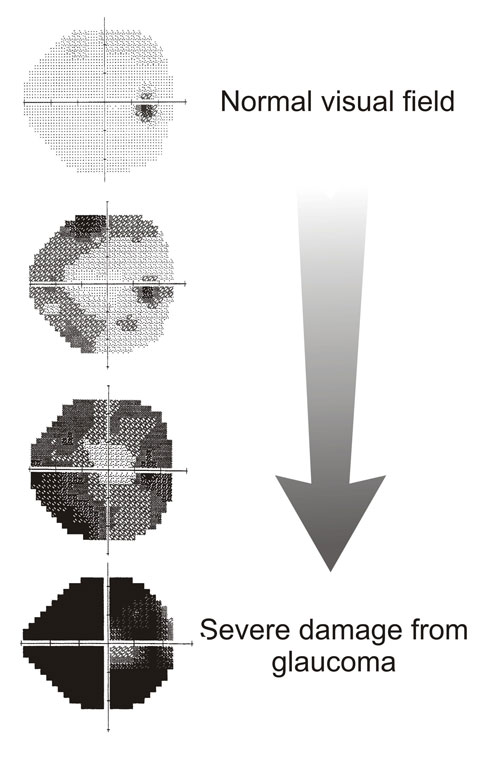
\includegraphics[width=0.75\linewidth]{images/Glaucoma.png}
    \caption{Typical visual field loss progression of glaucoma \citep{glaucoma4} }
    \label{fig: glaucoma progression}
\end{figure}

\begin{figure}[!h]
    \centering
    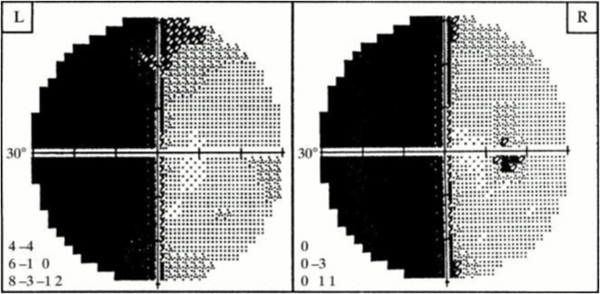
\includegraphics[width=0.75\linewidth]{images/hemanopia.png}
    \caption{Visual field map of left homonymous hemianopia \citep{hemanopia5}}
    \label{fig: hemanopia example}
\end{figure}

\begin{figure}
    \centering
    \includegraphics[width=6.5cm]{images/HFA.png}\hfill
    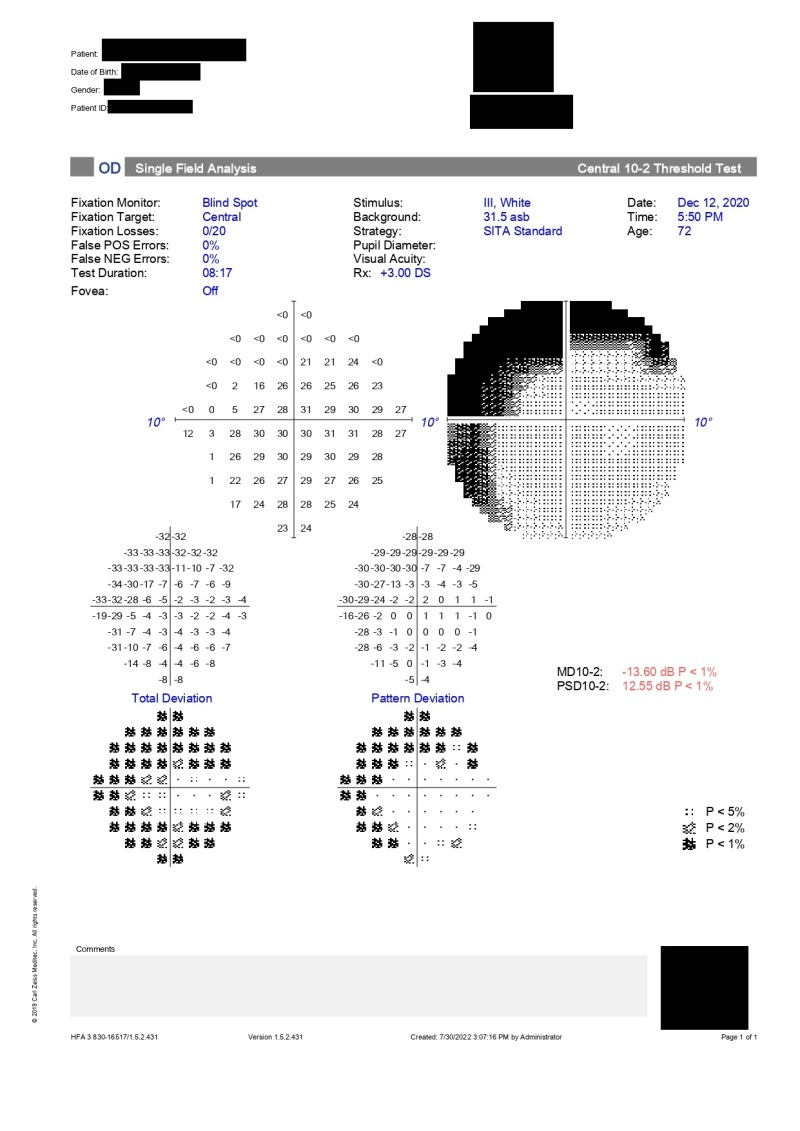
\includegraphics[width=6.5cm]{images/ExampleofVFTreport.png}
    \caption{Humphrey Field Analyser\citep{vftc} and sample HFA printout \citep{vftb}}
    \label{fig:HFA}
\end{figure}

\subsection{Simulation Sickness}

Simulator sickness, often referred to as “VR sickness”, is a well-documented side effect experienced by some users during immersive VR exposure. Symptoms include nausea, dizziness, eye strain, disorientation, and in some cases, headaches or fatigue. These effects are a result of sensory mismatch, particularly when visual motion does not align with vestibular or proprioceptive cues, such as in head movements or navigation \citep{vrb}.

A standardised way to measure these symptoms is through the Simulator Sickness Questionnaire (SSQ), developed by Kennedy et al., which quantifies sickness across three scales: nausea, oculomotor discomfort, and disorientation. SSQ is commonly administered before and after VR exposure to detect symptom onset and severity, and remains the standard for evaluating user tolerance in research and applied settings \citep{vra}.

The severity and onset of simulator sickness can vary based on multiple factors, including the duration of exposure, latency in the VR system, frame rate stability, field of view, and individual user susceptibility. For instance, lower frame rates and longer latencies tend to worsen symptoms, as does prolonged exposure to moving stimuli and scenes \citep{vrb}. Developers have responded by incorporating design practices that reduce discomfort, such as teleport-based movement, constrained camera motion, and shorter sessions, especially in health or research settings where user comfort is important.

\clearpage
\section{More on Implementation}

\subsection{Implementation Issues}
\label{SDK}
Due to the discontinued support for SDK SRanipal, we can no longer install the SDK, and we were forced to install a past student's work in order to get a Unity Editor that had pre-installed the SDK, which is why we used Unity Editor 2019. 

\subsection{In-depth hardware specifications}
\label{hardware}
According to the manufacturer's specifications \footnote{\href{https://www.tobii.com/products/integration/xr-headsets/device-integrations/htc-vive-pro-eye}{htc-vive-pro-eye specifications}}, the Vive Pro Eye provides:

\begin{itemize}
    \item A per-eye resolution of 1440 × 1600 pixels
 
    \item A field of view of approximately 110 degrees

    \item A refresh rate of 90Hz
\end{itemize}

These specifications contribute to a stable, high-fidelity VR experience that supports precise visual stimulus delivery, which is important for reducing simulator sickness and maintaining test validity.

The integrated eye-tracker supports a gaze accuracy of 0.5°–1.1° (visual angle) under ideal lighting and fit conditions, which is sufficient for fixation monitoring in a visual field context.



\subsection{Major Code Snippets}
\begin{lstlisting}[language={[Sharp]C}, caption = {Function that updates the stimulus coordinate} ]
    IEnumerator UpdateStimulusPosition()
{   
    if (count >= numCoords || gridPoints.Count == 0)
    {
        yield break;
    }

    Vector2 randomCoord = gridPoints[count];

    // Calculate new stimulus position based on grid
    float xStep = wallSize.x / (columns+1);
    float yStep = wallSize.y / (rows+1);

    float newX = wallStart.x + (randomCoord.x + rows/2 + 0.5f) * xStep;
    float newY = wallStart.y + (randomCoord.y + columns/2 + 0.5f) * yStep;

    Debug.Log(count + " " + newX + " " + newY);
    data.coords.Add(randomCoord);
    data.stimulusTime.Add(Time.time - testStartTime);
    
    // Update stimulus position
    stimulus.SetActive(true);
    // Debug.Log( stimulus is activated");
    // stimulus.transform.position = new Vector3(newX, newY, stimulus.transform.position.z);
    stimulus.transform.localPosition = new Vector3(newX, newY, 0);

    yield return StartCoroutine(WaitForTimer(flashDuration));
    // Debug.Log( stimulus is deactivated");
    stimulus.SetActive(false);
    

    yield return StartCoroutine(WaitForSpaceKey());

    count += 1;
}
\end{lstlisting}

\begin{lstlisting} [language={[Sharp]C}, caption = {JSON serialisation} ]
    IEnumerator StartStimulusTestSequence()
{
    
    while (count < numCoords && gridPoints.Count > 0)
    {
        yield return StartCoroutine(UpdateStimulusPosition());
    }

    Debug.Log("Stopping Now");
    testDuration = Time.time - testStartTime;
    Debug.Log($"Total Test Duration: {testDuration:0.00} seconds");
    centerPoint.GetComponent<MeshRenderer> ().material = red;
    stimulus.SetActive(false);
    
    data.testDuration = testDuration;
    data.numberOfPoints = numCoords;
    data.flashDuration = flashDuration;

    // Convert data to JSON format
    string json = JsonUtility.ToJson(data, true);

    // Save the JSON file
    string filePath = System.IO.Path.Combine(Application.dataPath, outputPath);

    // if doesnt exist, create
    Debug.Log(filePath);
    System.IO.Directory.CreateDirectory(filePath);
    System.IO.File.WriteAllText(System.IO.Path.Combine(filePath, "run_data.json"), json);

    eyeTracking.saveEyeJson();

    Debug.Log($"Run data JSON saved at: {filePath}");

    runPythonScript.RunPython();
    changeScene.GoToScene(0);
}
\end{lstlisting}

\begin{lstlisting} [language={[Sharp]C}, caption = {Python Runner} ]
    public void RunPython()
{

    if (string.IsNullOrEmpty(runPath))
    {
        UnityEngine.Debug.LogWarning("RunPythonScript: No runPath set. Skipping Python script.");
        return;
    }

    string pythonScript = Path.Combine(Application.dataPath, pythonScriptRelative);
    string args = $"\"{pythonScript}\" \"{runPath}\"";
    UnityEngine.Debug.Log("Running Python with args: " + args);


    ProcessStartInfo startInfo  = new ProcessStartInfo
    {
        FileName = pythonExecutable,
        Arguments = args,
        UseShellExecute = false,
        CreateNoWindow = true,
        RedirectStandardOutput = true, // True redirects output to unity
        RedirectStandardError = true // True Redirects errors
    };

    using (Process proc = Process.Start(startInfo))
    {
        string stdout = proc.StandardOutput.ReadToEnd();
        string stderr = proc.StandardError.ReadToEnd();
        proc.WaitForExit();

        UnityEngine.Debug.Log("STDOUT: " + stdout);
        if (!string.IsNullOrEmpty(stderr)){
            UnityEngine.Debug.LogWarning("STDERR: " + stderr);
        }
            
    }
}
\end{lstlisting}
\newpage
\section{More on Report Generation}
\label{report generation}
This section explains the automated post-test PDF generation process used in the VR-based visual field testing system. The Python script pdf\_generator.py is triggered from within Unity after each test session and compiles raw test data into a PDF report. The workflow involves five major stages:

\subsection{Data Parsing and Processing}
The script begins by loading two key JSON files:

\begin{itemize}
    \item run\_data.json (stimulus event data)
    \item eye\_tracking\_data.json (gaze samples)
\end{itemize}

\begin{lstlisting}[language={Python}]
    with open(file_path, "r") as file:
        data = json.load(file)
        ...
        reactionTime = np.array(data["reactionTime"])
        filter_arr = reactionTime != -1
        misc = {
            "testDuration": data["testDuration"],
            ...
            "averageReactionTime": np.mean(reactionTime[filter_arr]),
            }
\end{lstlisting}

From this, the script extracts:

\begin{itemize}
    \item The location and detection status of each stimulus
    \item Reaction time samples
    \item Gaze coordinates over time
    \item Timing of stimulus flashes
\end{itemize}

Additionally, it computes bounding limits (lim\_range) for plotting, and pre-processes the coordinates into a format that allows for easy lookup of detection frequency per point.

\subsection{Greyscale Figure Generation}
The script generates a custom greyscale visual field map. The number of times each stimulus was correctly detected (0–3) determines how densely filled a dot-pattern is placed within each grid cell, mimicking HVF-style greyscale charts.

\begin{lstlisting}[language={Python}]
    def plot_greyscale_dots(coords, detectedcount, lim_range):
        for i, coord in enumerate(coords):
        plot_cell_dotpattern(ax, coord[0], coord[1], detectedcount[i])
\end{lstlisting}

This method uses a nested dot grid: more misses result in denser black patterns. This approach avoids complex gradient scaling and gives the chart a more discrete, interpretable appearance.

\subsection{Gaze Density Figure Generation}
Gaze data is visualised using a kernel density estimation (KDE) technique to produce a density map of fixation concentration across the screen. This helps reviewers assess whether the participant maintained central fixation as instructed.

\begin{lstlisting}[language={Python}]
    def plot_gaze_contours(x, y, bins=50, lim_range):
        ...
        kernel = st.gaussian_kde(values)
        Z = np.reshape(kernel(positions), X.shape)
        plt.contourf(X, Y, Z, cmap='hot_r', levels=1000)
\end{lstlisting}

\subsection{Metrics Calculation}
The script computes key quantitative metrics used in the evaluation chapter:

\begin{itemize}
    \item False Positives: Button pressed while gaze is not on centre during a stimulus.
    \item Negatives: No response while gaze was correctly fixated.
    \item Center Fixation Percentage: Proportion of gaze points within central radius.
    \item Average Reaction Time: Mean time to respond to detected stimuli.
\end{itemize}

False positive detection is based on whether any gaze sample broke fixation during the stimulus flash, while the response was still logged as a detection.

\subsection{PDF Compilation}
The final step uses the reportlab library to generate a clean and professional-looking PDF report. The report includes:

\begin{itemize}
    \item Header Info: Name, test date, stimulus configurations
    \item Greyscale visual field map
    \item Gaze density map
    \item False positive scatter map
    \item Test metrics summary (reaction time, error rates, fixation\%)
\end{itemize}

Figures are converted to inline images using a buffer stream (fig\_to\_img) and arranged into a two-column layout using reportlab.platypus.Table. 

The resulting PDF mimics the layout and tone of traditional perimetry reports, ensuring readability for both clinicians and researchers.


\newpage
\section{More on Evaluation}
\subsection{In-depth details of Pilot Studies}
\label{sec:PilotStudiesDetails}

\subsubsection{Background Colour}:
A neutral gray background was selected to reduce glare, visual fatigue, and contrast distraction. This aligns with best practices in VR visual design, which recommend reducing high-contrast edges and overly bright environments to minimise discomfort and simulator sickness \citep{eval1}.

\subsubsection{Eye Isolation}:
While monocular testing in traditional perimetry often involves patching one eye, physical eye patches were found to interfere with headset comfort and eye-tracking reliability. Pilot testing suggested modifying the HMD by covering the lens of the untested eye, which provided an acceptable result. A software-based approach, achieved by ignoring data from one eye in future iterations, may be possible.

\subsubsection{Countdown Mechanism}:
A short pre-test countdown was implemented to help users settle into position and focus before stimulus onset. This is consistent with practices in psychophysical research, where brief acclimation periods are used to standardise pre-stimulus fixation \citep{eval2}.

\subsubsection{Brightness and Stimulus Size}:
Pilot study feedback indicated that moderately sized, high-contrast stimuli (white dots on a gray background) were both clearly visible and well-tolerated. Fine-tuned brightness calibration remains outside the current scope and is marked for future development.

\subsubsection{Reaction Time Allocation}:
Each trial includes flashing the stimulus briefly (0.05s) followed by a short window (0.7s) for user response. 

\subsubsection{Testing Duration}:
Test sessions lasting more than five minutes were reported to cause decreased attention and increased discomfort, especially among novice VR users. A test length of around 4–5 minutes was identified as optimal for maintaining concentration and minimizing fatigue. This observation is supported by studies that suggest limiting VR exposure to short sessions to avoid simulator sickness \citep{eval4}.

\subsubsection{Rest Time Duration}:
Participants were encouraged to remove the headset and rest between test sessions. Intermittent rest is known to reduce visual strain and improve sustained attention in prolonged or immersive visual tasks \citep{eval4}.

\clearpage
\subsection{User Study Introduction}
\begin{figure}
    \centering
    
\includegraphics[width=1\linewidth]{images//VFT study/p1.png}
\end{figure}
\clearpage

\begin{figure}
    \centering
    
\includegraphics[width=1\linewidth]{images//VFT study/p2.png}
\end{figure}
\clearpage

\begin{figure}
    \centering
    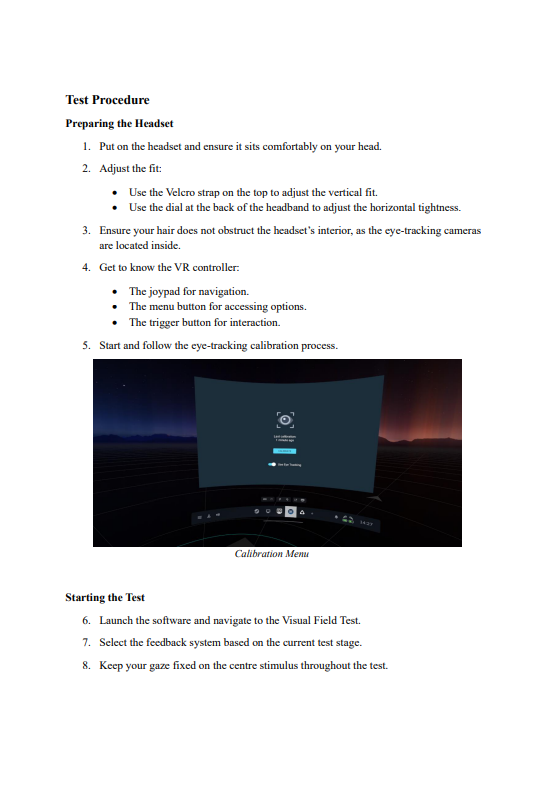
\includegraphics[width=1\linewidth]{images//VFT study/p3.png}
\end{figure}
\clearpage

\begin{figure}
    \centering
    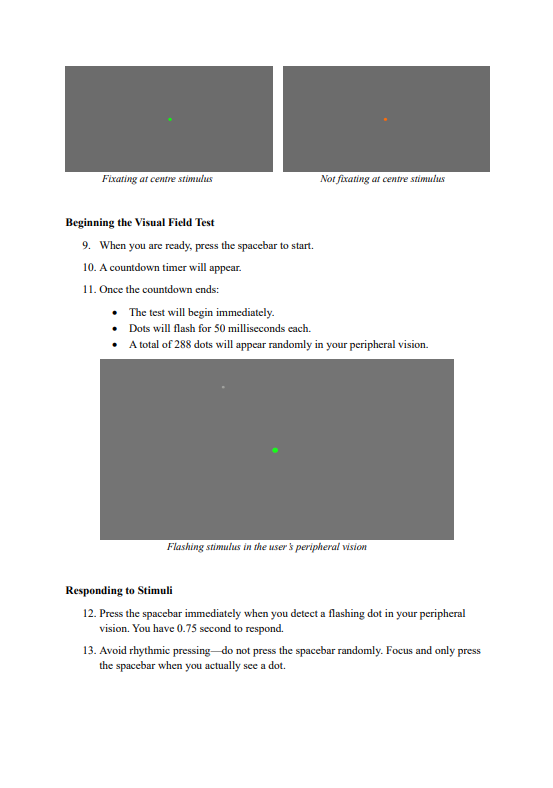
\includegraphics[width=1\linewidth]{images//VFT study/p4.png}
\end{figure}
\clearpage

\begin{figure}
    \centering
    
\includegraphics[width=1\linewidth]{images//VFT study/p5.png}
\end{figure}
\clearpage

\subsection{Ethics form}
\begin{figure}
    \centering
    
\includegraphics[width=1\linewidth]{images//Ethics form/p1.png}
\end{figure}
\clearpage

\begin{figure}
    \centering
    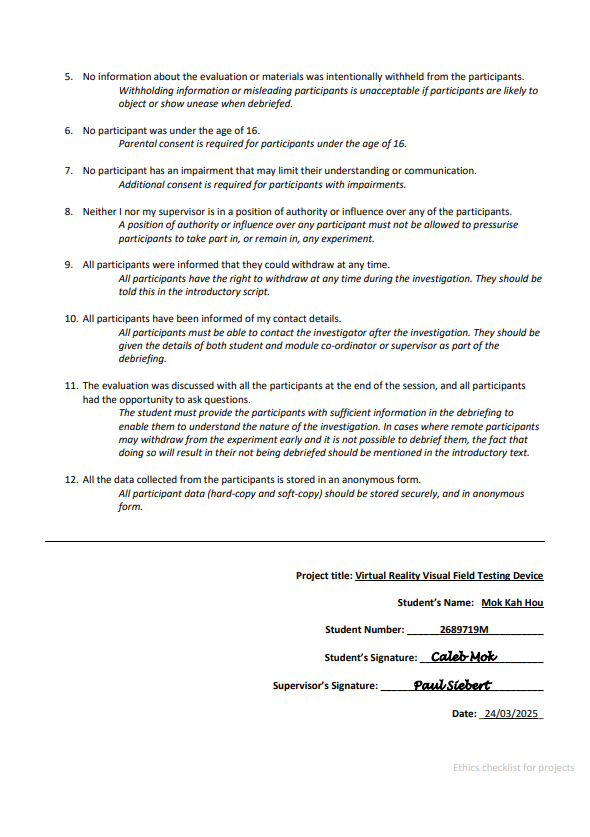
\includegraphics[width=1\linewidth]{images//Ethics form/p2.png}
\end{figure}
\clearpage

\subsection{Questionnaire}
\begin{figure}
    \centering
    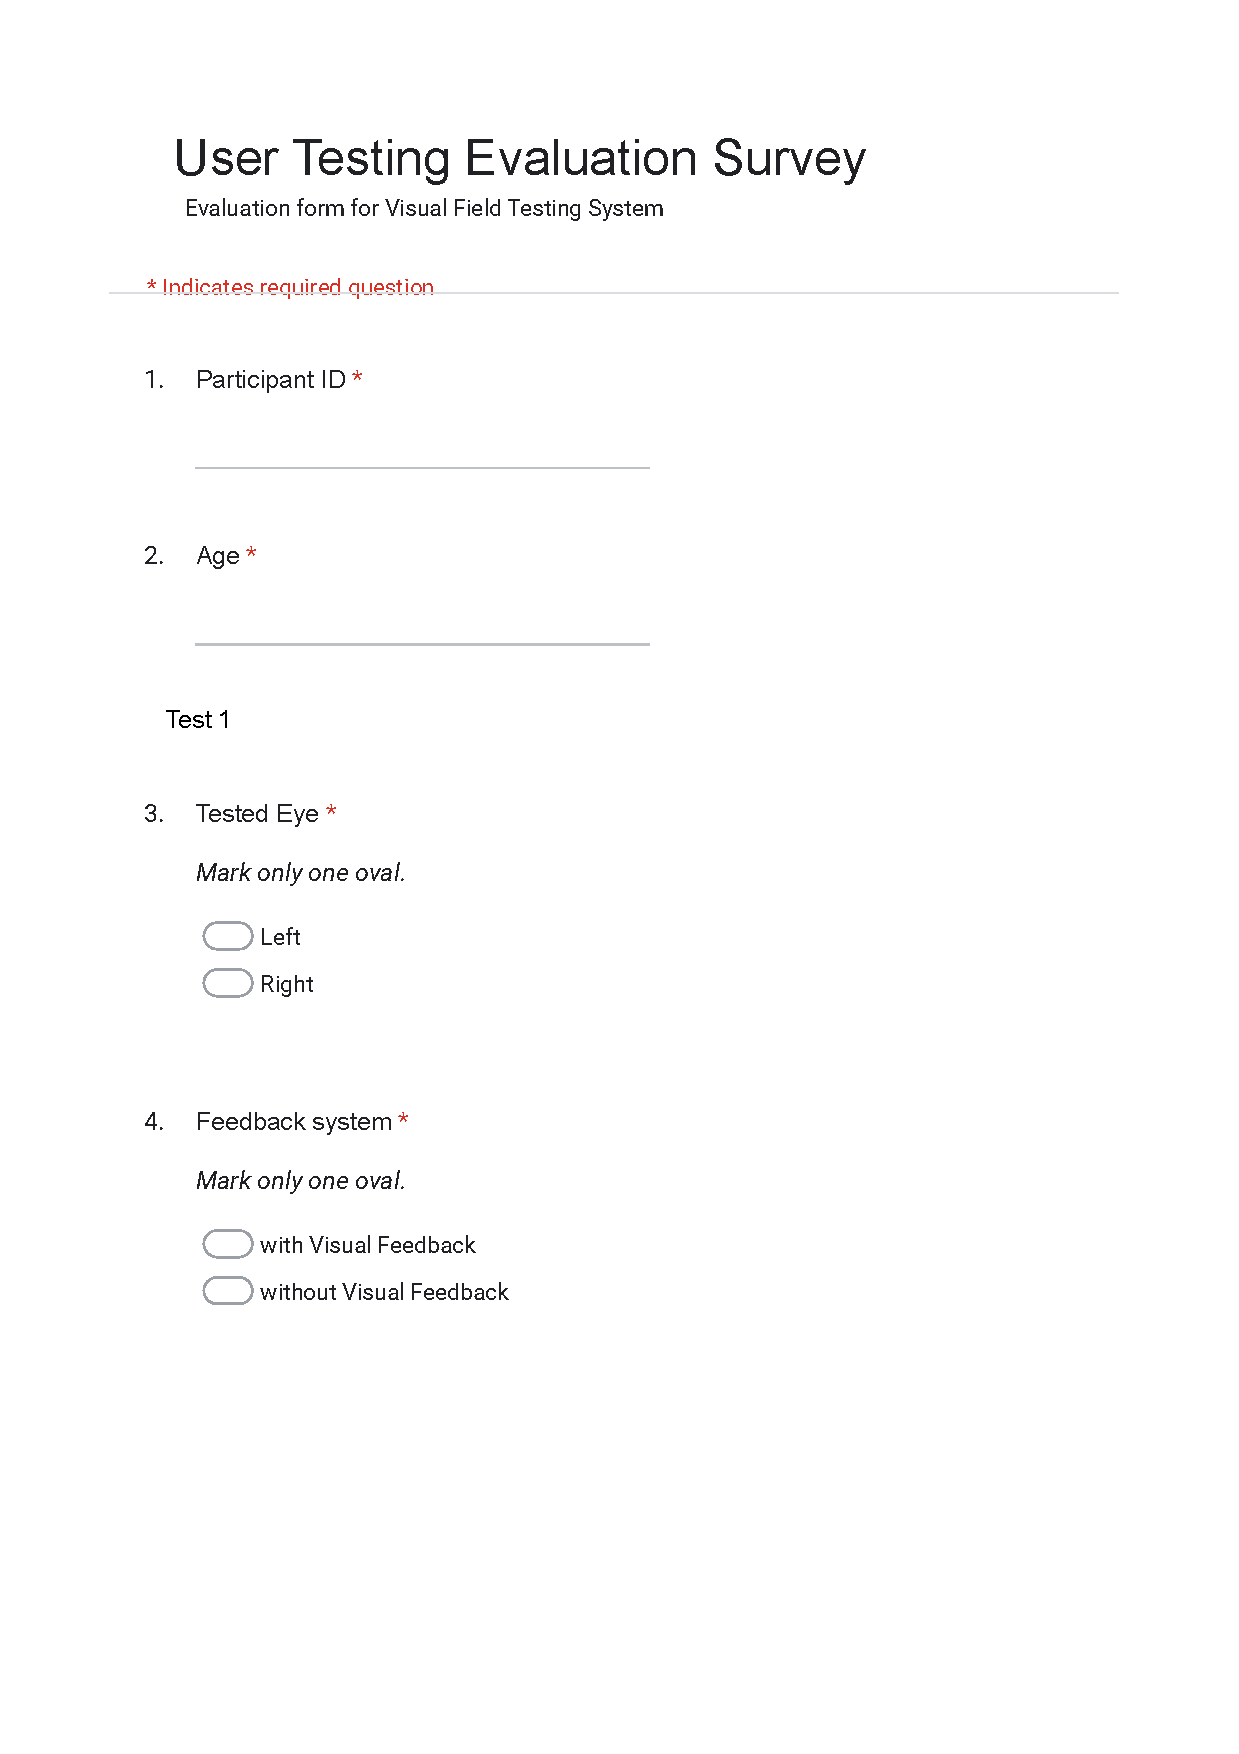
\includegraphics[page=1, width=1\linewidth]{images/User Testing Evaluation Form.pdf}
\end{figure}
\begin{figure}
    \centering
    \includegraphics[page=2, width=1\linewidth]{images/User Testing Evaluation Form.pdf}
\end{figure}
\begin{figure}
    \centering
    \includegraphics[page=3, width=1\linewidth]{images/User Testing Evaluation Form.pdf}
\end{figure}
\begin{figure}
    \centering
    \includegraphics[page=4, width=1\linewidth]{images/User Testing Evaluation Form.pdf}
\end{figure}
\begin{figure}
    \centering
    \includegraphics[page=5, width=1\linewidth]{images/User Testing Evaluation Form.pdf}
\end{figure}
\begin{figure}
    \centering
    \includegraphics[page=6, width=1\linewidth]{images/User Testing Evaluation Form.pdf}
\end{figure}
\begin{figure}
    \centering
    \includegraphics[page=7, width=1\linewidth]{images/User Testing Evaluation Form.pdf}
\end{figure}
\begin{figure}
    \centering
    \includegraphics[page=8, width=1\linewidth]{images/User Testing Evaluation Form.pdf}
\end{figure}
\begin{figure}
    \centering
    \includegraphics[page=9, width=1\linewidth]{images/User Testing Evaluation Form.pdf}
\end{figure}
\begin{figure}
    \centering
    \includegraphics[page=10, width=1\linewidth]{images/User Testing Evaluation Form.pdf}
\end{figure}
\begin{figure}
    \centering
    \includegraphics[page=11, width=1\linewidth]{images/User Testing Evaluation Form.pdf}
\end{figure}


\clearpage
\subsection{Latin Square}
\begin{figure}[!h]
    \centering
    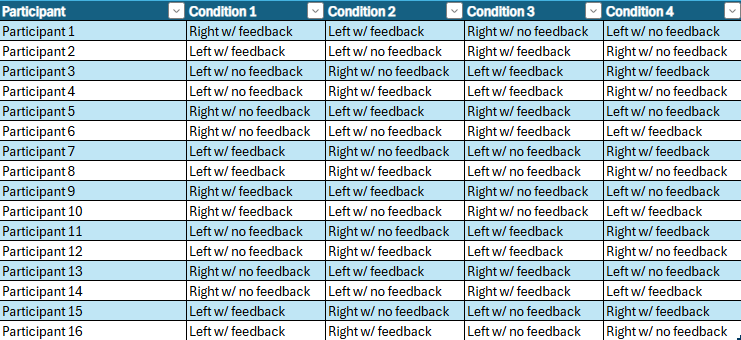
\includegraphics[width=1\linewidth]{images/LatinSquare.png}
    \caption{Latin Square for User Study}
    \label{LatinSquare}
\end{figure}

\subsection{Test Measure tables}
\begin{figure}[!h]
    \centering
    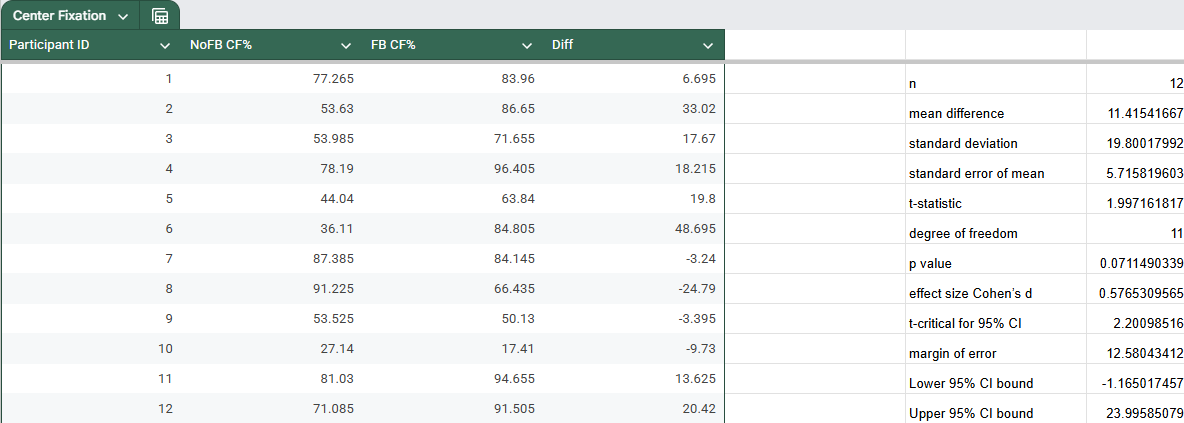
\includegraphics[width=1\linewidth]{images//CSFYP data analysis/Center Fixation Pecentage Analysis.png}
    \caption{Center Fixation Percentage Analysis}
    \label{fig:CFappendix}
\end{figure}

\begin{figure}[!h]
    \centering
    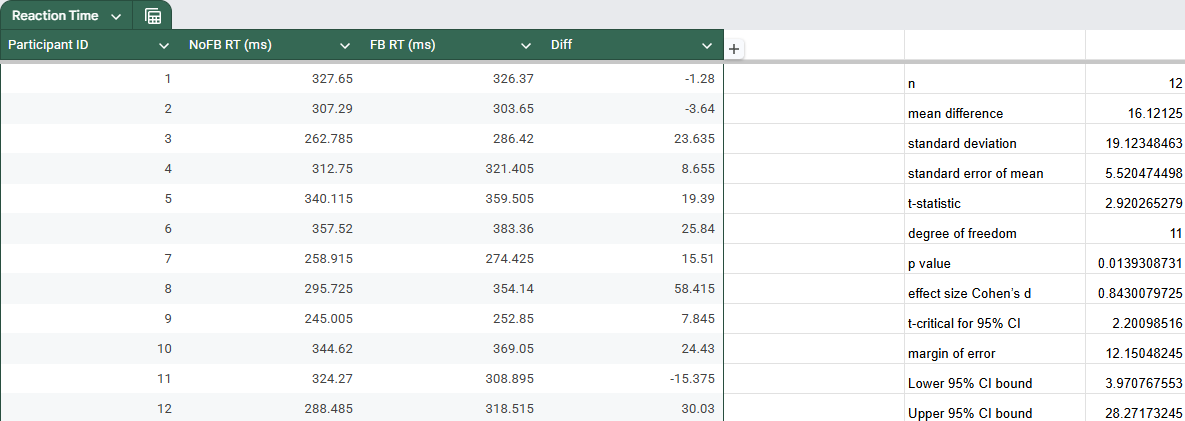
\includegraphics[width=1\linewidth]{images//CSFYP data analysis/Reaction Time Analysis.png}
    \caption{Reaction Time Analysis}
    \label{fig:RTappendix}
\end{figure}

\begin{figure}[!h]
    \centering
    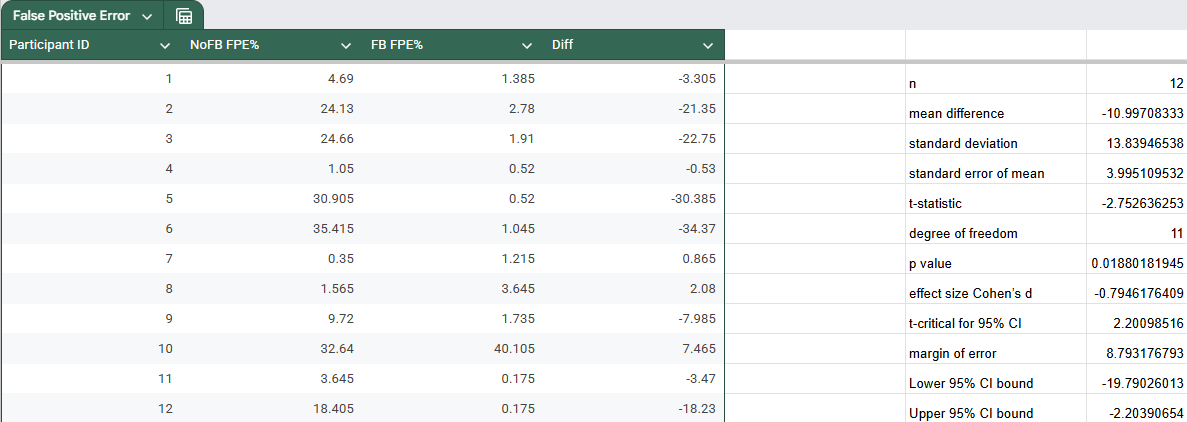
\includegraphics[width=1\linewidth]{images//CSFYP data analysis/False Positive Error Pecentage Analysis.png}
    \caption{False Positive Error Percentage Analysis}
    \label{fig:FPappendix}
\end{figure}

\begin{figure}[!h]
    \centering
    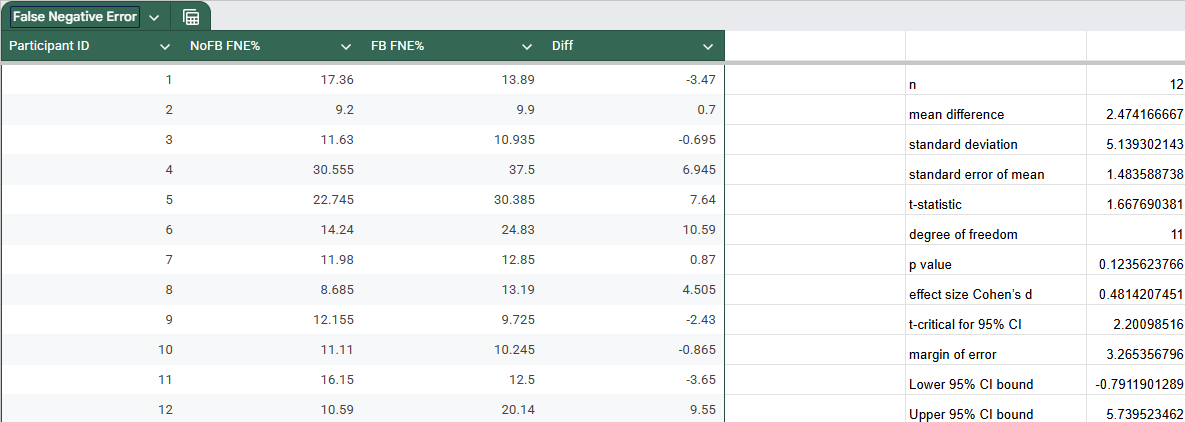
\includegraphics[width=1\linewidth]{images//CSFYP data analysis/False Negative Error Pecentage Analysis.png}
    \caption{Negative Error Percentage Analysis}
    \label{fig:FNappendix}
\end{figure}

\begin{figure}[!h]
    \centering
    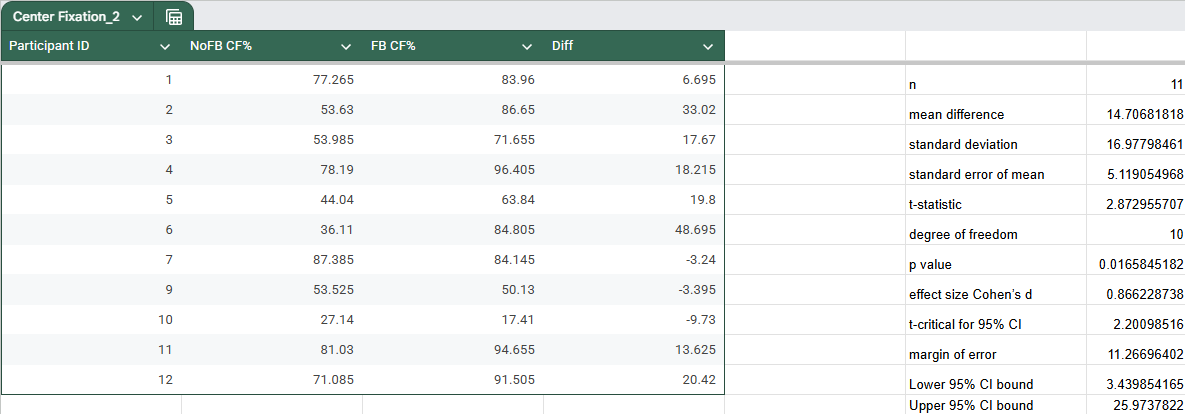
\includegraphics[width=1\linewidth]{images//CSFYP data analysis/Center Fixation Pecentage Analysis without Participant 8.png}
    \caption{Center Fixation Percentage without Participant 8}
    \label{fig:CFno8}
\end{figure}

\begin{figure}[!h]
    \centering
    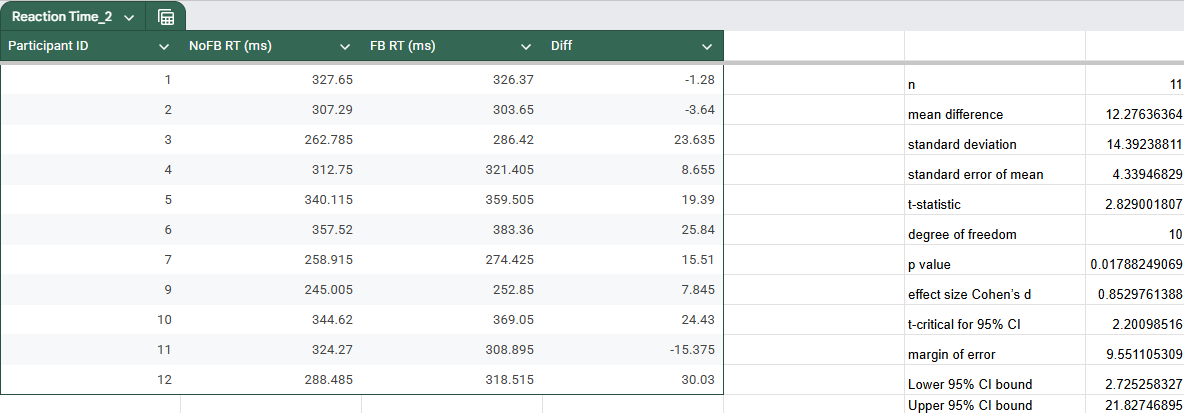
\includegraphics[width=1\linewidth]{images//CSFYP data analysis/Reaction Time Analysis without Participant 8.png}
    \caption{Reaction Time Analysis without Participant 8}
    \label{fig:RTappendixno8}
\end{figure}

\begin{figure}[!h]
    \centering
    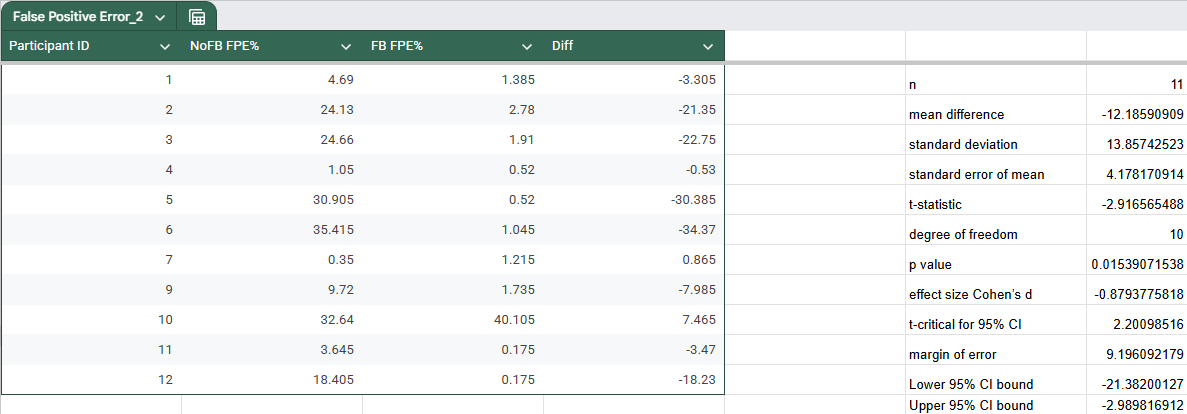
\includegraphics[width=1\linewidth]{images//CSFYP data analysis/False Positive Error Pecentage Analysis without Participant 8.png}
    \caption{False Positive Error Percentage Analysis without Participant 8}
    \label{fig:FPappendixno8}
\end{figure}

\begin{figure}[!h]
    \centering
    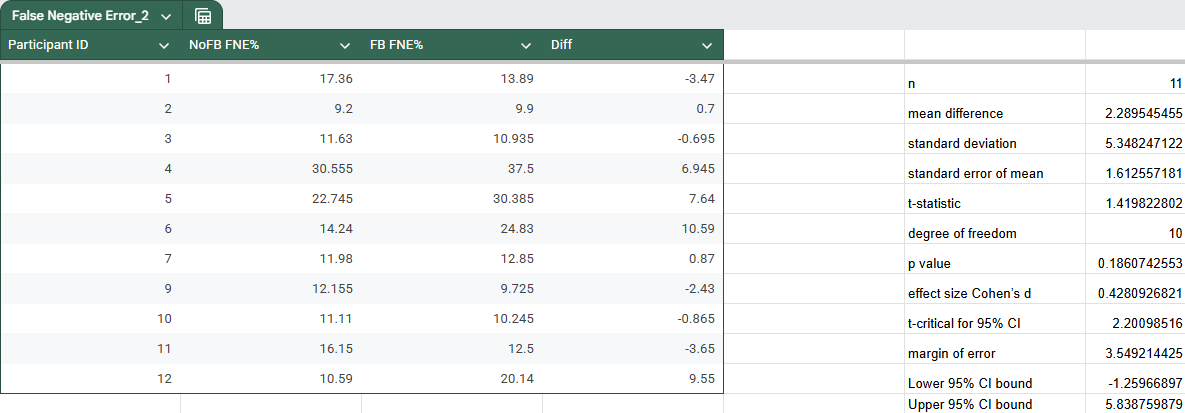
\includegraphics[width=1\linewidth]{images//CSFYP data analysis/False Negative Error Pecentage Analysis without Participant 8.png}
    \caption{Negative Error Percentage Analysis without Participant 8}
    \label{fig:FNappendixno8}
\end{figure}




\end{appendices}

%==================================================================================================================================
%   BIBLIOGRAPHY   

% The bibliography style is agsm (Harvard)
% The bibliography always appears last, after the appendices.

\bibliographystyle{agsm}

% Force the bibliography not to be numbered
\renewcommand{\thechapter}{0} 
\bibliography{l4proj}

\end{document}
